\documentclass[twocolumn]{IEEEtran}

\usepackage{macros}
\pdfminorversion=4

% The following packages will be automatically loaded:
% amsmath, amssymb, natbib, graphicx, url, algorithm2e
\begin{document}

\title{Model-free optimization of human preferences in stochastic systems}
\author{Cheng Jie$^\sharp$, Prashanth L A$^\dagger$, Michael Fu$^\$$, Steve Marcus$^\ddag$ and Csaba Szepesv\'ari$^\star$
\thanks{
$^\dagger$ Institute for Systems Research, University of Maryland, College Park, Maryland,
E-Mail: prashanth@isr.umd.edu,

$\sharp$ Department of Computer Science and Automation,
Indian Institute of Science, Bangalore,
E-Mail: shalabh@csa.iisc.ernet.in, 

$\$$ Robert H. Smith School of Business \& Institute for Systems Research,
University of Maryland, College Park, Maryland,
E-Mail: mfu@isr.umd.edu,

$\ddag$ Department of Electrical and Computer Engineering \& Institute for Systems Research,
University of Maryland, College Park, Maryland,
 E-Mail: marcus@umd.edu.

$\star$ Department of Computing Science,
University of Alberta,
 E-Mail: szepesva@cs.ualberta.ca.
}}
\maketitle


\begin{abstract}
Cumulative prospect theory (CPT) is known to model human decisions well, with substantial empirical evidence supporting this claim. 
CPT works by distorting probabilities and is more general than the classic expected utility and coherent risk measures. We bring this idea to a risk-sensitive reinforcement learning (RL) setting and design algorithms for both estimation and control.
The RL setting presents two particular challenges when CPT is applied: estimating the CPT objective requires estimations of the {\it entire distribution} of the value function and finding a {\it randomized} optimal policy.
The estimation scheme that we propose uses the empirical distribution to estimate the CPT-value of a random variable. We then use this scheme in the inner loop of a CPT-value optimization procedure that is based on the well-known simulation optimization idea of simultaneous perturbation stochastic approximation (SPSA).
We provide theoretical convergence guarantees for all the proposed algorithms and also 
illustrate the usefulness of CPT-based criteria in a traffic signal control application.
%empirically demonstrate the usefulness of our algorithms. 
\end{abstract}

% You may provide any keywords that you 
% find helpful for describing your paper; 
\begin{IEEEkeywords}
Prospect theory, reinforcement learning, stochastic optimization, simultaneous perturbation stochastic approximation.
\end{IEEEkeywords}

\section{Introduction}
\label{sec:introduction}

%!TEX root =  cpt-rl-icml.tex
% Since the beginning of its history, mankind has been deeply immersed in 
% 	designing and improving systems to serve human needs.
% Policy makers are busy with designing 
% 	systems that serve the education, transportation, economic, health and other 
% 	needs of the public,
% while private sector enterprises work hard at creating 
% 	and optimizing systems to better serve  
% 	specialized needs of their customers.
% While it has been long recognized that 
% 	understanding human behavior is a prerequisite 
% 	to best serving human needs \cite{Simon:1959kd},
% %	and the private sector has adopted this strategy a while ago \cite{}
% %	and the private sector quickly adopted this strategy,
% 	it is only recently that this approach is gaining a wider recognition.%
% \footnote{
% As evidence for this wider recognition in the public sector,
% we can mention a recent executive order of the White House
% calling for the use of behavioral science in public policy making, 
% or the establishment of the ``Committee on Traveler Behavior and Values'' in the Transportation
% Research Board in the US.}
% %Using Behavioral Science Insights to Better Serve the American People

In this paper we consider \emph{stochastic optimization problems}
where a designer optimizes the system 
to produce outcomes that are maximally aligned with the preferences of 
one or possibly multiple humans.
As a running example, consider traffic optimization where the goal is to maximize
travelers' satisfaction, a challenging problem 
%many may agree is  still inadequately addressed today, at least 
in big cities.
In this example, the outcomes (``return'') are travel times, or delays. 
To capture human preferences, the outcomes are mapped to a single numerical quantity.
%We will make the assumption that human preferences can 
%To create a single numerical quantity that faithfully captures human preferences, 
%a \emph{risk metrics}, mapping the random returns to some scalar deterministic quantity, is used.
While preferences of rational agents facing decisions with stochastic outcomes can be modeled using expected utilities,
i.e., the expectation of a nonlinear transformation, such as the exponential function, of the rewards or costs
\cite{NeuMo44,fishburn1970expectedutility}, 
	humans are subject to various emotional and cognitive biases.
	As the psychology literature points out, human preferences 
	are inconsistent with expected utilities regardless of what nonlinearities are used
	 \cite{allais53,ellsberg61,kahneman1979prospect}.
An approach that gained 
%Behavioral scientists use alternate approaches to model human preferences.
	strong support amongst psychologists, behavioral scientists and economists (cf. \cite{starmer2000developments,quiggin2012generalized})
	is based on Kahneman and Tversky's \cite{kahneman1979prospect} celebrated \emph{prospect theory} (PT),
	the theory that we will also base our models of human preferences on
	 in this work.
More precisely, we will use \emph{cumulative prospect theory} (CPT),
 	a later, refined variant of prospect theory due to Tversky and Kahneman \cite{tversky1992advances}, 
	which superseded prospect theory.
CPT generalizes expected utility theory in that in addition to having a utility function transforming
	the outcomes, another function is introduced which distorts the probabilities in the cumulative distribution function.
As compared to prospect theory, CPT is monotone with respect to stochastic dominance, a property
	that is thought to be useful and more consistent with human preferences.
	%\footnote{See Appendix \ref{sec:appendix-cpt-intro} for an introduction to PT/CPT and an explanation of why expected utility theory is inconsistent with human preferences.}
	
\if0	

Popular approaches that use such risk metrics include the exponential utility formulation 
(cf. \cite{borkar2010learning}) that implicitly controls the variance.
An alternative is a to consider constrained formulations 
with explicit constraints on the variance of the return (cf. \cite{tamar2012policy,Prashanth13AC}). 
Another constraint alternative is to bound a coherent risk measure such as Conditional Value-at-Risk (CVaR), 
while minimizing the usual cost objective (cf. \cite{borkar2010risk,prashanth2014policy}).  

The risk metrics underlying the above-mentioned works 
are based on the assumption that human decision makers are rational and/or consistent.
While this may hold in certain restricted settings, a large body of literature indicates that humans are neither rational,
\todoc{Add literature supporting this. At least three books:)}
nor consistent (which, in fact, is an unsurprising fact, at least in the experience of the authors of the paper).
In other words, traditional approaches are based on the belief that optimizing the expected utility (EU) is appealing for human subjects. However, there is substantial evidence that this is not case - see 
the survey article \cite{starmer2000developments} and Chapter 4 of the book \cite{quiggin2012generalized}. In particular, the aforementioned references describe the Allais and Ellsberg paradoxes popular among economists for arguing against EU. 
Thus, if the goal is to produce outcomes that are best aligned with human preferences,
an alternative approach is required.
A singularly popular and successful approach in behavioral science and economics
is based on \textit{prospect theory (PT)} \cite{kahneman1979prospect} 
and its later enhancement, the so-called \textit{cumulative prospect theory} (CPT) \cite{tversky1992advances}.
CPT is a rank dependent expected utility model \cite{quiggin2012generalized} that incorporates decision weights to distort probabilities. 
The suitability of this approach to model human decision making (and thus preferences) has been widely documented \cite{prelec1998probability}, \cite{wu1996curvature}, \cite{conlisk1989three}, \cite{camerer1989experimental}, \cite{camerer1992recent}, \cite{harless1992predictions}, \cite{sopher1993test}, \cite{camerer1994violations}, \cite{gonzalez1999shape}, \cite{abdellaoui2000parameter}.
PT/CPT has been applied in a variety of domains, for e.g., healthcare \cite{lenert1999associations},  seismic design \cite{goda2008application}, transportation \cite{gao2010adaptive},\cite{fujii2004drivers}, \cite{ramming2001network}, online auctions \cite{weinberg2005exploring}, insurance  \cite{machina1995non} and finance \cite{barberis1999prospect}, \cite{epstein1989substitution}, \cite{epstein1991substitution}.
\fi

% \tikzset{
%   pobl/.style={
%     inner sep=0pt, outer sep=0pt, fill=#1,
%   },
%   pobl gron/.style n args={2}{
%     pobl=#1, rounded corners=#2,
%   },
%   pics/person/.style n args={3}{
%     code={
%       \node (-corff) [pobl=#1, minimum width=.25*#2, minimum height=.375*#2, rotate=#3, pic actions] {};
%       \node (-pen) [minimum width=.3*#2, circle, pobl=#1, outer sep=.01*#2, anchor=south, rotate=#3, pic actions] at (-corff.north) {};
%       \node (-coes dde) [pobl gron={#1}{1pt}, anchor=north west, minimum width=.12125*#2, minimum height=.25*#2, rotate=#3, pic actions] at (-corff.south west) {};
%       \node [pobl=#1, anchor=north, minimum width=.12125*#2, minimum height=.15*#2, rotate=#3, pic actions] at (-coes dde.north) {};
%       \node (-coes chwith) [pobl gron={#1}{1pt}, anchor=north east, minimum width=.12125*#2, minimum height=.25*#2, rotate=#3, pic actions] at (-corff.south east) {};
%       \node [pobl=#1, anchor=north, minimum width=.12125*#2, minimum height=.15*#2, rotate=#3, pic actions] at (-coes chwith.north) {};
%       \node (-braich dde) [pobl gron={#1}{.75pt}, minimum width=.075*#2, minimum height=.325*#2, outer sep=.0064*#2, anchor=north west, rotate=#3, pic actions] at (-corff.north east)  {};
%       \node [pobl=#1, minimum width=.05*#2, minimum height=.2*#2, outer sep=.0064*#2, anchor=north west, rotate=#3, pic actions] at (-corff.north east) {};
%       \node (-braich chwith) [pobl gron={#1}{.75pt}, minimum width=.075*#2, minimum height=.325*#2, outer sep=.0064*#2, anchor=north east, rotate=#3, pic actions] at (-corff.north west) {};
%       \node [pobl=#1, minimum width=.0375*#2, minimum height=.2*#2, outer sep=.0064*#2, anchor=north east, rotate=#3, pic actions] at (-corff.north west) {};
%       \node (-fit person) [fit={(-pen.north) (-braich dde.east) (-coes chwith.south) (-braich chwith.west)}] {};
%       %\node (-pwy) [below=25pt of -fit person, every pin] {\tikzpictext};
%       %\draw [every pin edge] (-fit person) -- (-pwy);
%     },
%   },
% }
% \tikzstyle{block} = [draw, fill=white, rectangle,
%    minimum height=3em, minimum width=6em]
% \tikzstyle{sum} = [draw, fill=white, circle, node distance=1cm]
% \tikzstyle{input} = [coordinate]
% \tikzstyle{output} = [coordinate]
% \tikzstyle{pinstyle} = [pin edge={to-,thin,black}]
% 
% \begin{figure}[h]
% \centering
% \scalebox{0.65}{\begin{tikzpicture}
% \node [block,fill=blue!20, minimum height=4em,] (world) {\makecell{\large\bf Stochastic \\\large\bf System}}; 
% \node [block,fill=red!20, below=2.5cm of world] (agent) {\makecell{\large\bf Optimization \\\large\bf Algorithm}}; 
% \node [circle,fill=brown!50!black,right=2cm of world,label=above:{\bf Reward}] (tmp) {};
% \coordinate [below left=2.5cm of world] (tmp2);
% \coordinate [below right=1cm of agent] (belowagent);
% 
% \draw [->,thick] (world)  -| (tmp) |-   (agent);
% \draw [->,thick] (agent)  -| (tmp2) |-   (world);
% %\draw [->] (agent) --   (world);
% \draw pic (person)  [right =3cm of tmp] {person={blue}{50pt}{0}};
% \coordinate [right=2.8cm of tmp] (tmp3);
% \coordinate [right=3.3cm of tmp] (tmp31);
% \coordinate [right=1cm of tmp3] (belowhuman);
% \coordinate [right=3.5cm of tmp3] (tmp4);
% \draw [->,thick] (tmp) --   (tmp3);
% \draw [-,thick,dotted] (tmp31)  -- node[below right=0.1cm and 0.5cm] {\textbf{Preferences}} (belowhuman) --  (tmp4);
% \draw [->,thick,dotted] (tmp4)  |-  (belowagent) -|  (agent.south);
% \end{tikzpicture}}
% \caption{Operational flow of a human-based decision making system
% }
% \label{fig:flow}
% \end{figure}
% %\begin{tikzpicture}
%   %[
%     %every pin edge/.append style={latex-, shorten <=-2.5pt},
%   %]

%
%In the realm of sequential decision making under uncertainty, we propose a CPT-based risk measure.  In particular,  
%The current RL solutions cannot handle distortions and my current work is to develop both prediction and control schemes for probabilistically distorted MDPs.
%
%\todop[inline]{Add refs for distorted weights}
%In this paper, we consider a risk measure based on \textit{cumulative prospect theory} (CPT) \cite{tversky1992advances}, which is a non-coherent and non-convex measure that is well known among psychologists and economists to be a good model for human decision-making systems, with strong empirical support. In this paper, we incorporate CPT-based criteria into the classic objective \textit{value function} in a reinforcement learning framework. Intuitively this combination is appealing because it taps into the notion of how humans evaluate outcomes and also, a CPT objective leads to a randomized policy, which although harder to estimate often leads to more intuitively appealing behavior, as illustrated via an example below and also the numerical experiments later.

%%%%%%%%%%%%\
\subsection*{Our contributions\footnote{A preliminary version of this paper was published in ICML 2016 \cite{la2016cumulative}. In comparison to the conference version, this paper includes additional theoretical results, formal proofs of convergence of both estimation and optimization algorithms, additional experiments and a revised presentation.}}

To the  best of our knowledge, we are the first to incorporate CPT into an online stochastic optimization framework. Although on the surface the combination may seem straightforward, in fact there are many challenges that arise from trying to optimize a CPT objective in the stochastic optimization framework, as we will soon see. 
In this short summary, we outline these challenges as well as our approach to addressing them. 

The first challenge stems from the fact that the CPT-value assigned to a random variable is defined through a nonlinear transformation of the cumulative distribution function associated with the underlying random variable (see \cref{sec:cpt-val} for the definitions). 
Hence, even the problem of estimating the CPT-value given a random sample is challenging.
%\textbf{\textit{Prediction:}} In the case of the classic value function, which is an expectation, a simple sample mean can be used for estimation, facilitating the use of temporal difference type algorithms. On the other hand, 
%CPT-value   involves a distribution that is distorted using non-linear weight functions and hence, 
%requires that the \textit{entire} distribution to be estimated.\\ 
%\textit{Solution:} 
In this paper, we consider a natural quantile-based estimator and analyze its behavior.
Under certain technical assumptions, we prove consistency and give sample complexity bounds, the latter based on the
 Dvoretzky-Kiefer-Wolfowitz (DKW) theorem.
As an example, we show that the sample complexity for estimating the CPT-value 
for Lipschitz probability distortion weight functions is  $O\left(\frac1{\epsilon^2}\right)$, which coincides with the canonical rate for Monte Carlo-type schemes and is thus unimprovable. Since weight functions that fit well to human preferences are only  \holder continuous, we also consider this case and find that (unsurprisingly) the sample complexity  degrades to $O\left(\frac1{\epsilon^{2/\alpha}}\right)$ where $\alpha\in (0,1]$ is the weight function's \holder exponent.
%However, for weight functions which are only \holder continuous with exponent $\alpha \in (0,1)$,
%Thus, at least in this case, 
%At the same time, 
% while \holder continuous with constant $\alpha$ results in a rate  $O\left(\frac1{\epsilon^{2/\alpha}}\right)$, for achieving a $\epsilon$-close estimate.\\

Our results on estimating CPT-values form the basis of the algorithms that we propose to maximize CPT-values based on interacting either with a real environment or with a simulator. 
% We set up this problem as an instance of policy search: 
We consider a smooth parameterization of the CPT-value and propose two algorithms for updating the CPT-value parameter. The first algorithm is a stochastic gradient scheme that uses two-point randomized gradient estimators, borrowed from simultaneous perturbation stochastic approximation (SPSA) \cite{spall}\footnote{A second-order CPT-value optimization scheme based on SPSA is described in \cite{la2016cumulative}.}. 
% We employ a three-point SPSA-based Hessian estimator proposed in \cite{bhatnagar2015simultaneous}. 
%\textbf{\textit{Control:}} 
%Designing algorithms in order to find a \textit{CPT-optimal} policy is challenging because CPT-value is a non-coherent and non-convex risk measure that does not lend itself to dynamic programming approaches such as value/policy iteration due to the lack of a ``Bellman equation''. 
%Thus, it is necessary to design new simulation optimization scheme that use sample CPT-value estimates to optimize the policy, which is generally \textit{randomized}. While classic simulation optimization settings usually have a zero mean noise in function evaluations, our setting one has to tradeoff simulation cost with the bias in a manner such that the resulting policy optimization scheme cancels the bias effect and converges. \\
%\textit{Solution:} 
%Using the well-known idea of simultaneous perturbation stochastic approximation (SPSA) from the \textit{simulation optimization} literature \cite{fu2015handbook}, we propose and analyze a gradient method for CPT value optimization in sequential decision making problems
%under uncertainty.
The second algorithm is a gradient-free method that is adapted from \cite{chang2013simulation}. The idea is to use a reference model that eventually concentrates on the global minimum and then empirically approximate this reference distribution well-enough. The latter is achieved via natural exponential families in conjunction with Kullback-Leibler (KL) divergence to measure the ``distance'' from the reference distribution. 
Guaranteeing convergence of the aforementioned CPT-value optimization algorithms is challenging because only  \emph{biased} estimates of the CPT-value are available. We propose a particular way of controlling the arising bias-variance tradeoff and establish convergence for all proposed algorithms.
% We establish that our algorithm converges to a globally CPT-value optimal policy (assuming it exists).
% Here a new challenge arises, which is that we can only feed the two-point randomized gradient estimator with \emph{biased} estimates of the CPT-value. To guarantee convergence, we propose a particular way of controlling the arising bias-variance tradeoff.

%Since SPSA by default assumes that the unbiased point-estimates of the optimization objective are available, which
%is not the case in our problem, we extend the analysis of SPSA to handle the case when the optimization objective estimates are noisy, with controlled bias.
%
%We derive the condition that specifies the rate at which the number of samples for predicting the CPT-value should increase such that the bias of CPT-value estimates vanishes asymptotically (see (A3) later).
%
%, while the second is a Newton algorithm that also uses SPSA-based estimates of the gradient and also the Hessian. We remark again that, unlike traditional settings for SPSA, our estimates for CPT-value have a non-zero (albeit controlled) bias. We establish that our algorithms converge to a locally CPT-value optimal policy. 

% \todoc[inline]{Im not sure what to do with the following para, as we havent talked about RL and position our work as CPT + sto-opt}

\textit{Related work.}
Various risk measures have been proposed in the literature, e.g., mean-variance tradeoff \cite{markowitz1952portfolio}, exponential utility \cite{Arrow1971}, value at risk (VaR) and conditional value at risk (CVaR) \cite{rockafellar2000optimization}. A large body of literature involves risk-sensitive optimization in the context of Markov decision processes (MDPs).   
The stochastic optimization context of this paper translates to a risk-sensitive reinforcement learning (RL) problem, and it has been observed in earlier works that risk-sensitive RL is generally hard to solve. 
For instance, in \cite{Sobel82VD}, \cite{filar1989variance} and \cite{mannor2013algorithmic}, the authors provide NP-hardness results for finding a globally variance-optimal policy in discounted and average reward MDPs.
Solving CVaR constrained MDPs is equally complicated (cf. \cite{borkar2010risk,prashanth2014policy}). In contrast, incorporating CPT-based criteria incurs extra sample complexity in estimation as compared to that of the classic sample mean estimator for expected value, while the optimization schemes based either on SPSA or model-based parameter search \cite{chang2013simulation} that we propose converge at the same rate as that of their expected value counterparts. 
% Finally, we point out that the CPT-value is a generalization of all the risk measures above in the sense that one can recover these particular risk measures such as VaR and CVaR by appropriate choices of the distortions used in the definition of the CPT-value.
In the context of an abstract MDP setting, a CPT-based risk measure has been proposed in \cite{lin2013stochastic}. Unlike \cite{lin2013stochastic},
\begin{inparaenum}[\it (i)]
\item we do not assume a nested structure for the CPT-value, %\eqref{eq:cpt-mdp} 
and this implies the lack of a Bellman equation for our CPT measure;
\item we do not assume model information, i.e., we operate in a more general stochastic optimization setting;
\item we develop both estimation and optimization algorithms with convergence guarantees for the CPT-value function.
\end{inparaenum}
More recently, the authors in \cite{aditya2016weighted} incorporate CPT-based criteria into a multi-armed bandit setting, while employing the estimation scheme that we proposed in the shorter version of this paper \cite{la2016cumulative}. 

The rest of the paper is organized as follows: 
In Section~\ref{sec:cpt-val}, we define the notion of CPT-value for a general random variable.
In Section~\ref{sec:cpt-sampling}, we
describe the empirical distribution-based scheme for estimating the CPT-value of any random variable. In Section \ref{sec:cpt-control}, we present gradient-based algorithms for optimizing the CPT-value. 
%Next, in Section \ref{sec:mras}, we present a gradient-free model-based algorithm for CPT-value optimization in an MDP. 
We provide proofs of convergence for all the proposed algorithms in Section~\ref{sec:convergence}.
In Sections~\ref{sec:expts-simple} and \ref{sec:expts}, we present simulation experiments for synthetic and traffic signal control problems, respectively. Finally, in Section~\ref{sec:conclusions} we provide our concluding remarks.


%%%%%%%%%%%%%5
\section{CPT-value}
\label{sec:cpt-val}
%!TEX root =  cpt-rl-icml.tex

For a real-valued random variable $X$, we introduce a ``CPT-functional'' that replaces the traditional expectation operator. 
%Subsequently, we specialize $X$ to be the return of stochastic shortest path problem. 
%\subsection{General definition}
%\label{sec:cptdef}
The functional, denoted by $\C$,
indexed by
$u=(u^+,u^-)$, $w=(w^+,w^-)$, where $u^+,u^-:\R\rightarrow \R_+$ and $w^+,w^-:[0,1] \rightarrow [0,1]$ are continuous,
with $u^+(x)=0$ when $x\le 0$ and $u^-(x)=0$ when $x\ge 0$ (see assumptions (A1)-(A2) in Section \ref{sec:cpt-sampling} for precise requirements on $u$ and $w$),
 is defined as 
\begin{align}
\C_{u,w}(X) &= \intinfinity w^+\left(\Prob{u^+(X)>z}\right) dz\nonumber \\
&\quad - \intinfinity w^-\left(\Prob{u^-(X)>z}\right) dz\,. \label{eq:cpt-general}
\end{align}
For notational convenience, when $u,w$ are fixed, we drop the dependence on them and use $\C(X)$ to denote the CPT-value of $X$. Note that when $w^+,w^-$
and $u^+$ ($-u^-$), when restricted to the positive (respectively, negative) half line, 
are the identity functions, and we let $(a)^+ = \max(a,0)$, $(a)^- = \max(-a,0)$,
$\C(X) = \intinfinity \Prob{X>z} dz -  \intinfinity \Prob{-X>z} dz = \EE{ (X)^+ } - \EE{ (X)^- }$, showing the connection to expectations.
%\cref{fig:u} shows an example of the utility functions $u= (u^+,u^-)$ and how they relate to each other, while \cref{fig:w} shows an example of a typical weight function.

 \begin{figure}[h]
   \centering
\tabl{c}{
%\includegraphics[width=3.8in]{utility.png}}
   \scalebox{0.5}{\begin{tikzpicture}
   \begin{axis}[width=13cm,height=6.5cm,legend pos=south east,
          %  grid = major,         
            axis lines=middle,
           % grid style={dashed, gray!30},
            xmin=-5,     % start the diagram at this x-coordinate
            xmax=5,    % end   the diagram at this x-coordinate
            ymin=-4,     % start the diagram at this y-coordinate
            ymax=4,   % end   the diagram at this y-coordinate
           % axis background/.style={fill=white},
            ylabel={\large\bf Utility},
            xlabel={\large\bf Gains},
            x label style={at={(axis cs:4.7,-0.8)}},
            y label style={at={(axis cs:-0.8,4.8)}},
            xticklabels=\empty,
            yticklabels=\empty
            ]
           \addplot[name path=cptplus,domain=0:5, green!35!black, very thick,smooth] 
              {pow(abs(x),0.8)}; 
            \addplot[name path=cptminus,domain=-5:0, red!35!black,very thick,smooth] 
              {-2*pow(abs(x),0.7)}; 
               \addplot[domain=-5:5, blue, thick]           {x}; 
               
               \path[name path=diagplus] (axis cs:0,0) -- (axis cs:5,5);
 			  \path[name path=diagminus] (axis cs:-5,-5) -- (axis cs:0,0);
                \path[name path=xaxisplus] (axis cs:0,0) -- (axis cs:5,0);
                 \path[name path=xaxisminus] (axis cs:-5,0) -- (axis cs:0,0);
                 \path[name path=yaxisplus] (axis cs:0,0) -- (axis cs:0,5);
                 \path[name path=yaxisminus] (axis cs:0,-5) -- (axis cs:0,0);
 
 \addplot [orange!40]  fill between[of= diagminus and yaxisminus];
 \addplot [cyan!20]  fill between[of= diagplus and xaxisplus];
 
 \node at (axis cs:  -3.7,-0.45) {\large\bf Losses};
 \node at (axis cs:  4,2.5) {\large $\bm{u^+}$};
 \node at (axis cs:  -1,-3) {\large $\bm{-u^-}$};
% \node at (axis cs:  2.5,-2.5) {\large\bf Baseline};
%\draw[-{>[scale=2.5,
%          length=5,
%          width=3]},thick] (axis cs:2,-2) -- (axis cs:0,0);
   \end{axis}
   \end{tikzpicture}}}\\[1ex]
\caption{An example of a utility function. A reference point on the $x$ axis serves as the point of separating gains and losses.
For losses, the disutility $-u^-$ is typically convex, for gains, the utility $u^+$ is typically concave; 
they are always non-decreasing and both of them take on the value of zero at the reference point.}
\label{fig:u}
\end{figure}


In the definition, $u^+, u^-$ are utility functions corresponding to gains ($X \ge 0$) and losses ($X \le 0$), respectively,
where zero is chosen as a somewhat arbitrary ``reference point'' to separate gains and losses.
Handling losses and gains separately is a salient feature of CPT, and this addresses the tendency of humans to play safe with gains and take risks with losses. % - see Fig \ref{fig:u}. 
To illustrate this tendency, 
consider a scenario where one can either earn \$$500$ with probability (w.p.) $1$ or earn \$$1000$ w.p. $0.5$ and nothing otherwise. 
The human tendency is to choose the former option of a certain gain. 
If we flip the situation, i.e., a certain loss of \$$500$ or a loss of \$$1000$ w.p. $0.5$, 
then humans choose the latter option.  
This distinction of playing safe with gains and taking risks with losses is captured by a concave gain-utility
$u^+$ and a convex disutility $-u^-$, cf. \cref{fig:u}.
%In contrast, the traditional value function makes no such distinction between gains and losses.  

\begin{figure}[h]
\centering
\tabl{c}{
%\includegraphics[width=8cm]{results/Probability_weighting_function.jpg}
  \scalebox{0.65}{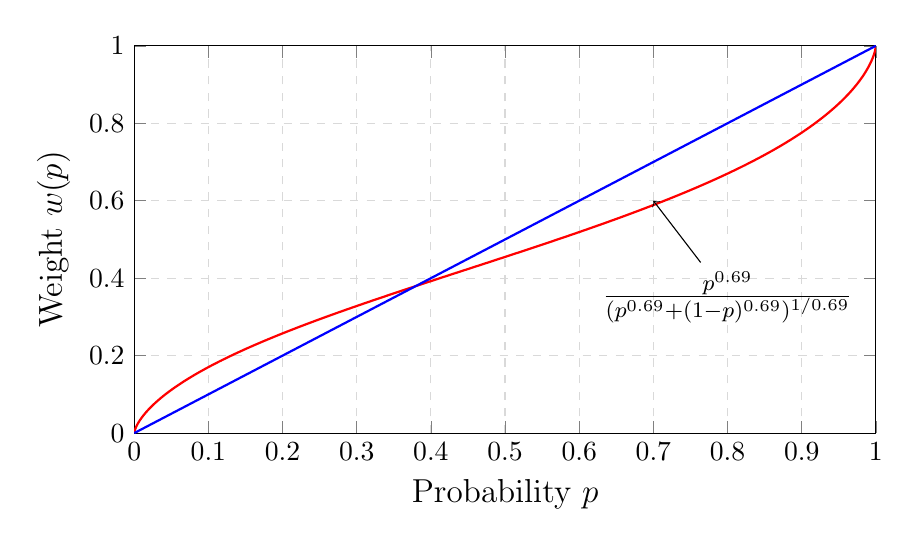
\begin{tikzpicture}
  \begin{axis}[width=11cm,height=6.5cm,legend pos=south east,
           grid = major,
           grid style={dashed, gray!30},
           xmin=0,     % start the diagram at this x-coordinate
           xmax=1,    % end   the diagram at this x-coordinate
           ymin=0,     % start the diagram at this y-coordinate
           ymax=1,   % end   the diagram at this y-coordinate
           axis background/.style={fill=white},
           ylabel={\large Weight $\bm{w(p)}$},
           xlabel={\large Probability $\bm{p}$}
           ]
          \addplot[domain=0:1, red, thick,smooth,samples=1500] 
             {pow(x,0.69)/pow((pow(x,0.69) + pow(1-x,0.69)),1.44)}; 
             \node at (axis cs:  0.8,0.35) (a1) {\large $\bm{\frac{p^{0.69}}{(p^{0.69}+ (1-p)^{0.69})^{1/0.69}}}$};           
             \draw[->] (a1) -- (axis cs:  0.7,0.6);
                 \addplot[domain=0:1, blue, thick]           {x};                      
  \end{axis}
  \end{tikzpicture}}\\[1ex]
}
\caption{An example of a weight function.
A typical CPT weight function inflates small, and deflates large probabilities, capturing the 
tendency of humans doing the same when faces with decisions of uncertain outcomes.
}
\label{fig:w}
\end{figure}

The functions $w^+, w^-$, called the weight functions, capture the idea that humans deflate high-probabilities and inflate low-probabilities.
For example, humans usually choose a stock that gives a large reward, e.g., 
one million dollars w.p. $1/10^6$ over one that gives \$$1$ w.p. $1$ and the reverse when signs are flipped. 
Thus the value seen by a human subject is nonlinear in the underlying probabilities -- an observation backed by strong empirical evidence \cite{tversky1992advances,Barberis:2012vs}.  
%In contrast, the expected utility is linear in the underlying probabilities. 
As illustrated with $w=w^+=w^-$ in Fig \ref{fig:w}, the weight functions are continuous, non-decreasing and  have the range $[0,1]$ with $w^+(0)=w^-(0)=0$ and $w^+(1)=w^-(1)=1$. 
In \cite{tversky1992advances}, the authors recommend $w(p) = \frac{p^{\eta}}{{(p^{\eta}+ (1-p)^{\eta})}^{1/\eta}}$, while in \cite{prelec1998probability}, the author recommends $w(p) = \exp(-(-\ln p)^\eta)$, with $0 < \eta <1$. In both cases, the weight function has an inverted-s shape.
% which is seen to be a good fit from empirical tests on human subjects - see \cite{conlisk1989three}, \cite{camerer1989experimental}, \cite{camerer1992recent}, \cite{harless1992predictions}, \cite{sopher1993test}, \cite{camerer1994violations}, \cite{gonzalez1999shape}, \cite{abdellaoui2000parameter}.  
\if0
Weight functions can explain nonlinear probability distortions, as illustrated by the following example: \\
\textit{\textbf{[Stock 1]}} This investment results in a gain of \$$10$ with probability (w.p.) $0.1$ and a loss of \$$500$ w.p. $0.9$. The expected return is \$$-449$, but this does not necessarily imply that ``human'' investors' evaluation of the stock is \$$-449$. Instead, it is very likely that the humans evaluate it to a higher value, e.g. \$$-398$ ($=$ gain w.p. $0.2$ and loss w.p. $0.8$).\footnote{See Table 3 in \cite{tversky1992advances} to know why such a human evaluation is likely.}\\
\textit{\textbf{[Stock 2]}} loss of \$$10$ w.p. $0.9$, gain \$$500$ w.p. $0.1$. Expected return: \$$41$; Human evaluation: \$$92$ ($=$ loss w.p. $0.8$).\\
\textit{\textbf{[Stock 3]}} loss of \$$10$ w.p. 0.1, gain \$$500$ w.p. $0.9$. Expected return: \$$449$; Human evaluation: \$$398$ ($=$ loss w.p. $0.2$). 
\fi



%A few remarks are in order.
\begin{remark}\textit{(RL applications)}
%The CPT-value, as defined in \eqref{eq:cpt-general}, has several applications in RL. In general, 
For any RL problem setting, one can define the return for a given policy and then apply a CPT-functional on the return. For instance, with a fixed policy, the random variable (r.v.) $X$ could be the total reward in a stochastic shortest path problem or the infinite horizon cumulative reward in a discounted MDP or the long-run average reward in an MDP.
 %- See Appendix \ref{sec:cpt-ssp} for one such application. 
\end{remark}


%\subsection{Application: Stochastic Shortest Path}
%We consider a stochastic shortest path (SSP) problem with states $\S=\{0,\ldots,\L\}$, where $0$ is a special reward-free absorbing state.  A randomized policy $\pi$ is a function that maps any state $s\in \S$ onto a probability distribution over the actions $\A(s)$ in state $s$. As is standard in policy gradient algorithms, we parameterize $\pi$ and assume it is continuously differentiable in its parameter $\theta \in \R^d$.  
%An \textit{episode} is a simulated sample path using policy $\theta$ that starts in state $x^0\in \S$, visits $\{x_1,\ldots, x_{\tau-1}\}$ before ending in the absorbing state $0$, where $\tau$ is the first passage time to state $0$.
%Let $D^\theta(s^0)$ be a random variable (r.v) that denote the total reward from an episode, defined by
%$$ D^\theta(s^0) = \sum\limits_{m=0}^{\tau-1} r(s_m,a_m), $$
%where the actions $a_m$ are chosen using policy $\theta$ and $r(s_m, a_m)$ is the single-stage reward in state $s_m\in \S$ when action $a_m \in \A(s_m)$ is chosen. 
%
%Instead of the traditional RL objective for an SSP of maximizing the expected value $\E (D^\theta(s^0))$, 
%we adopt the CPT approach and aim to solve the following problem: 
%$$ \max_{\theta \in \Theta} \C(D^\theta(s^0)),$$
%where $\Theta$ is the set of admissible policies that are \textit{proper}\footnote{A policy $\theta$ is proper if $0$ is recurrent and all other states are transient for the Markov chain underlying $\theta$. It is standard to assume that policies are proper in an SSP setting - cf. \cite{bertsekas1995dynamic}.} and the CPT-value function $\C(D^\theta(s^0))$ is defined as
%\begin{align}
%\C(D^\theta(s^0))& = \intinfinity w^+(P(u^+(D^\theta(s^0)))>z) dz \nonumber
%\\&- \intinfinity w^-(P(u^-(D^\theta(s^0)))>z) dz. \label{eq:cpt-mdp}
%\end{align}

\begin{remark}\textit{(Generalization)}
As noted earlier, the CPT-value is a generalization of mathematical expectation. 
It is also possible to get \eqref{eq:cpt-general} to coincide with risk measures (e.g. VaR and CVaR) by appropriate choice of weight functions.
\end{remark}

%\begin{remark}\textit{(Sensitivity)}
%\todoc{I think this is really hard to defend.
%Since the derivative of the weight function at zero is very high (even zero),
%the CPT value is hugely sensitive (even more so than the expected value) to error
%in low probabilities. We should remove this remark.
%}
%Traditional EU-based approaches are sensitive to modeling errors as illustrated in the following example: 
%Suppose stock $\cal{A}$ gains \$$10000$ w.p $0.001$ and loses nothing w.p. $0.999$, while stock $\cal B$ surely gains $11$. With the classic value function objective, it is optimal to invest in stock $\cal B$ as it returns $11$,  while $\cal A$ returns $10$ in expectation (assuming utility function to be the identity map). Now, if the gain probability for stock $\cal A$ was $0.002$, then it is no longer optimal to invest in stock $\cal B$ and investing in stock $A$ is optimal.
%Notice that a very slight change in the underlying probabilities resulted in a big difference in the investment strategy and a similar observation carries over to a multi-stage scenario (see the house buying example in the numerical experiments section). 
 %%A randomized policy that $50$\% in stock $\cal A$ and the rest in a risk-free asset is less sensitive to the error in under-estimating the loss probability. 
%
%Using CPT makes sense because it inflates low probabilities and thus can account for modeling errors, especially considering that model information is unavailable in practice.
%Note also that in MDPs with expected utility objective, there exists a deterministic policy that is optimal. However, with CPT-value objective, the optimal policy is \textit{not necessarily} deterministic - See also the organ transplant example on pp. 75-81 of \cite{lin2013stochastic}. 
%\end{remark}




%%%%%%%%%%%%%%%%%%%%%%%%%%%%%%%%%%%%%%%%%%%%%%%%%%%%%%%%%%%%%%
%%%%%%%%%%%%%%%%%%%%%%%%%%%%%%%%%%%%%%%%%%%%%%%%%%%%%%%%%%%%%%
%%%%%%%%%%%%%%%%%%%%%%%%%%%%%%%%%%%%%%%%%%%%%%%%%%%%%%%%%%%%%%
%%%%%%%%%%%%%%%%%%%%%%%%%%%%%%%%%%%%%%%%%%%%%%%%%%%%%%%%%%%%%%
%%%%%%%%%%%%%%%%%%%%%%%%%%%%%%%%%%%%%%%%%%%%%%%%%%%%%%%%%%%%%%
%%%%%%%%%%%%%%%%%%%%%%%%%%%%%%%%%%%%%%%%%%%%%%%%%%%%%%%%%%%%%%
%%%%%%%%%%%%%%%%%%%%%%%%%%%%%%%%%%%%%%%%%%%%%%%%%%%%%%%%%%%%%%
%%%%%%%%%%%%%%%%%%%%%%%%%%%%%%%%%%%%%%%%%%%%%%%%%%%%%%%%%%%%%%

\section{Prediction of CPT-value} 
\label{sec:cpt-sampling}

%!TEX root =  cpt-rl-icml.tex
%For the sake of notational simplicity, we let $X$ denote the r.v. $X^\theta$, i.e., where the parameter $\theta$ is assumed to be fixed for the purpose of CPT-value estimation in this section. \todoc{If we remove the $X^\theta$ business from above, this sentence can be removed.}

We devise a scheme for estimating CPT-value $\C(X)$  given only samples from the distribution of $X$.
 %and show that, under each of the aforementioned assumptions, our estimator (presented next) converges almost surely. 
%We also provide sample complexity bounds, assuming that the utility functions are bounded.
%\paragraph{On integrability}
Before diving into the details of CPT-value estimation, let us discuss the conditions necessary for the CPT-value to be well-defined.
Observe that the first integral in \eqref{eq:cpt-general}, i.e., 
$\int_0^{+\infty} w^+\left(\Prob{u^+(X)>z}\right) d z$
may diverge even if the first moment of random variable $u^+(X)$ is finite. 
For example, suppose $U$ has the tail distribution function
$\Prob{U>z}  = \frac{1}{z^2}, z\in [1, +\infty),$
 and $w^+(z)$ takes the form $w(z) = z^{\frac{1}{3}}$. Then, the first integral in \eqref{eq:cpt-general}, i.e.,
$
\int_1^{+\infty}  z^{-\frac{2}{3}}\, dz
$
does not even exist. A similar argument applies to the second integral in \eqref{eq:cpt-general}.

To overcome the integrability issues, we assume that the weight functions $w^+, w^-$ satisfy one of the following assumptions for continuous valued r.v.s: 

\noindent\textbf{Assumption (A1).}  
The weight functions $w^+, w^-$ are H\"{o}lder continuous with common order $\alpha$ and constant $H$, i.e.,
$\sup_{x \neq y} \frac{| w{\pm}(x) - w{\pm}(y) |}{| x-y |^{\alpha}} \leq H$, $\forall x,y \in [0,1]$.
 Further,
there exists $ \gamma \le \alpha$ such that (s.t.)
$\int_0^{+\infty} \mathbb{P}^{\gamma} (u^+(X)>z) dz < +\infty$ and $\int_0^{+\infty} \mathbb{P}^{\gamma} (u^-(X)>z) dz < +\infty$,
where $\mathbb{P}^{\gamma}(\cdot) = \left(\mathbb{P}(\cdot)\right)^{\gamma}$.

\noindent\textbf{Assumption (A1').}  The weight functions $w^+, w^-$ are Lipschitz with common constant $L$, and 
$u^+(X)$ and $u^-(X)$ both have bounded first moments.

\begin{proposition}
\label{prop:cpt-finite}
Under (A1) or (A1'), the CPT-value $\C(X)$ as defined by \eqref{eq:cpt-general} is finite. 
\end{proposition}
\begin{proof}
See Section \ref{sec:holder-proofs}.
\end{proof}

%Under both (A1) a we provide asymptotic consistency for the CPT-value estimator presented in the next section. 
(A1') even though it implies (A1), is a useful special case because it does away with additional assumptions required to establish asymptotic consistency under (A1). For the theoretical results, we also require the following assumption on the utility functions:

\noindent\textbf{Assumption (A2).}  The utility functions $u^+$ and $-u^-$ are continuous and strictly increasing on their support $\R^+$ and $\R^-$, respectively.

Finally, we also analyze the setting where $X$ is a discrete valued r.v. Such a setting is common in practice and carries the additional advantage that, under a local Lipschitz assumption on the distribution of $X$, one gets better sample complexity as compared to those under (A1) and (A1'). 

%The above assumption ensures that the CPT-value as defined by \eqref{eq:cpt-general} is finite - see Proposition 
%\ref{prop:Holder-cpt-finite} in Section \ref{sec:holder-proofs} for a formal proof.


%%%%%%%%%%%%%%%%%%%%%%%%%%%%%%%%%%%%%%%%%%%%%%%%%%%%%%%%%%%%%%
\subsection{CPT-value estimation using quantiles}
Let $\xi^+_{k}$ and $\xi^-_{k}$ denote the $k$th quantiles of the r.v.s $u^+(X)$ and $u^-(X)$, respectively. 
Then, it can be seen that (see Proposition \ref{prop:holder-quantile} in Section \ref{sec:holder-proofs})
\begin{align}
&\lim_{n \rightarrow \infty} \sum_{i=1}^{n} \xi^+_{\frac{i}{n}} \left(w^+\left(\frac{n+1-i}{n}\right)- w^+\left(\frac{n-i}{n}\right) \right) \nonumber\\
&= \int_0^{+\infty} w^+\left(\Prob{u^+(X)>z}\right) dz.\label{eq:holder-quant-motiv}
\end{align}
A similar claim holds with $u^-(X)$, $\xi^-_{k}, w^-$ in place of  $u^+(X)$, $\xi^+_{\alpha}, w^+$, respectively. 

However, we do not know the distribution of $u^+(X)$ or $u^-(X)$ and hence, we next present a procedure that uses order statistics for estimating quantiles and this in turn assists estimation of the CPT-value along the lines of \eqref{eq:holder-quant-motiv}. The estimation scheme is presented in Algorithm \ref{alg:holder-est}.

\begin{algorithm}
\caption{CPT-value estimation}
\label{alg:holder-est}
\begin{algorithmic}[1]
    \State {\bf Input:}  samples $X_1,\ldots,X_n$ from the distribution of $X$.
%\State Calculate $u^+(X_{[1]}),\ldots u^+(X_{[n]}).$
\State Arrange the samples in ascending order and label them as follows: 
$X_{[1]}, X_{[2]}, \ldots ,X_{[n]}$. 
%Since we assume $u^+$ is increasing (see (A2) below),  $u^+(X_{[1]}),\ldots ,u^+(X_{[n]})$ are in ascending order.
%\State Use $u^+(X_{[i]}), i\in \mathbb{N}\cap (0,n)$ as an approximation for the $\frac{i}{n} th$ quantile of $u^+(X)$, i.e, $\xi_{\frac{i}{n}}, i\in \mathbb{N}\cap (0,n)$.
\State Let
\vspace{-0.5ex}
\begin{align*}
\overline \C_n^+&:=\sum_{i=1}^{n} u^+(X_{[i]}) \left(w^+\!\left(\frac{n+1-i}{n}\right)\!-\! w^+\!\left(\frac{n-i}{n}\right) \right),\\
\overline \C_n^-&:=\sum_{i=1}^{n} u^-(X_{[i]}) \left(w^-\left(\frac{i}{n}\right)- w^-\left(\frac{i-1}{n}\right) \right). 
\end{align*}

\vspace{-0.5ex}
\State Return $\overline \C_n =\overline \C_n^+ - \overline \C_n^-$.
\end{algorithmic}
\end{algorithm}

Consider the special case when $w^+(p)=w^-(p)=p$ and $u^+$ ($-u^-$), when restricted to the positive (respectively, negative) half line, are the identity functions. In this case, the CPT-value estimator $\overline \C_n$ coincides with the sample mean estimator for regular expectation. 

Notice that the CPT estimator $\overline \C_n$ in Algorithm \ref{alg:holder-est} can be written equivalently as follows:
\begin{align}
\overline \C_n = \intinfinity w^+\left(1-{\hat F_n}^+\left(x\right)\right)  dx \!-\! \intinfinity w^-\left(1-{\hat F_n}^-\left(x\right)\right)  dx.
\label{eq:cpt-est-appendix}
\end{align}
The above relation holds because 
%\todoc{The hats should be on $F$ only, as in $\hat{F}^+$ as opposed to $\hat{F^+}$.}
\begin{align*}
&\sum_{i=1}^{n} u^+\left(X_{[i]}\right) \left(w^+\left(\frac{n+1-i}{n}\right) - w^+\left(\frac{n-i}{n}\right)\right) \\
&= \sum_{i=1}^{n-1} w^+\left(\frac{n-i}{n}\right) \left(u^+\left(X_{[i+1]}\right) - u^+\left(X_{[i]} \right)\right) + u^+(X_{[1]})\\
&=  \int_0^{\infty} w^+\left(1-\hat{F}^+_n\left(x\right)\right) dx, \text{ and }\\
&\sum_{i=1}^{n} u^-\left(X_{[i]}\right) \left(w^-\left(\frac{i}{n}\right) - w^-\left(\frac{i-1}{n}\right)\right)\\
& =  \int_0^{\infty} w^-\left(1-\hat{F}^-_n\left(x\right)\right) dx, 
\end{align*}
where $\hat{F}^+_n\left(x\right)$ and $\hat{F}^-_n\left(x\right)$ are the empirical distributions of $u^+\left(X\right)$
and $u^-\left(X\right)$, respectively.


%%%%%%%%%%%%%%%%%%%%%%%%%%%%%%%%%%%%%%%%%%%%%%%%%%%%%%%%%%%%%%
\subsection{Results for \holder and Lipschitz continuous weights}

%In order to ensure the integrability of the CPT-value \eqref{eq:cpt-general}, we make the following assumption:\\[1ex]



%\subsubsection*{Main results}
%We make the following assumptions on the utility functions:\\[1ex]

%For the sample complexity results below, we require (A2'), while (A2) is sufficient to prove asymptotic consistency.
\begin{proposition}(\textbf{Asymptotic consistency})
\label{prop:holder-asymptotic}
Assume (A1), (A2),\\
\begin{inparaenum}[\bfseries (i)]
\item $F^+(\cdot)$ and $F^-(\cdot)$, the respective distribution functions of $u^+(X)$ and $u^-(X)$, 
are Lipschitz continuous on the respective intervals $(0,+\infty)$, and 
$(-\infty, 0)$. \\
\item Utility functions $u^+, u^-$ satisfy 
$$\lim\limits_{n\rightarrow\infty}\frac{u^+(X_{[n]})}{n^{\alpha}}\rightarrow 0 \text{ and }\lim\limits_{n\rightarrow\infty}\frac{u^-(X_{[n]})}{n^{\alpha}}\rightarrow 0 \text{ a.s.}.$$
\end{inparaenum}
Then, we have 
\begin{align}
\overline \C_n
\rightarrow
\C(X)
 \text{   a.s. as } n\rightarrow \infty
\end{align}
where $\overline \C_n$ is as defined in Algorithm \ref{alg:holder-est} and $\C(X)$ as in \eqref{eq:cpt-general}.
\end{proposition}
The conditions in item (ii) above is satisfied by popular distribution choices such as Gaussian and exponential, while heavy-tailed distributions, e.g. Cauchy, do not.
\begin{proof}
See Section \ref{sec:holder-proofs}. 
\end{proof}
%Our next result concerns the rate at which the estimate $\overline \C_n$ converges to the CPT-value $\C(X)$. 
%Under (A2') stated below, 
Under an additional assumption on the utility functions,
our next result shows that $O\left(\frac{1}{\epsilon^{2/\alpha}}\right)$ number of samples are sufficient to get a
high-probability estimate of the CPT-value that is $\epsilon$-accurate.
\begin{proposition}(\textbf{Sample complexity.})
\label{prop:holder-dkw}
Assume (A1), (A2) and also that the utilities $u^+(X)$ and $u^-(X)$ are bounded above by $M<\infty$ w.p. 1. Then, $\forall \epsilon >0, \delta >0$, we have
$$
\Prob{\left |\overline \C_n- \C(X) \right| \leq  \epsilon } >1- \delta\text{     ,} \forall n \geq \frac{1}{2}\ln\left(\frac{4}{\delta}\right)
\left(\frac{HM}{\epsilon}\right)^{\frac{2}{\alpha}}.$$
\end{proposition}

\begin{corollary}
\label{cor:holder-dkw}
Under the conditions of Proposition \ref{prop:holder-dkw}, we have
$$
\E \left|\overline \C_n- \C(X) \right|  \le    \frac{\left(8HM\right) \Gamma\left(\alpha/2\right)}{n^{\alpha/2}},$$
where $\Gamma(\cdot)$ is the gamma function.
\end{corollary}

\begin{proof}
%
%%Notice the the following equivalence:
%%$$\sum_{i=1}^{n-1} u^+(X_{[i]}) (w^+(\frac{n-i}{n}) - w^+(\frac{n-i-1}{n})) =  \int_0^M w^+(1-\widehat{F^+_n}(x)) dx, $$
%%and also,
%%$$\sum_{i=1}^{n-1} u^-(X_{[i]}) (w^-(\frac{n-i}{n}) - w^-(\frac{n-i-1}{n})) =  \int_0^M w^-(1-\widehat{F^-_n}(x)) dx, $$
%%
%%where $\widehat{F^+_n}(x)$ and $\widehat{F^-_n}(x)$ are the empirical distribution functions (EDFs) of $u^+(X)$
%%and $u^-(X)$, defined as follows:
%%\begin{align}
%%{\widehat F_n}^+(x)=&\frac{1}{n} \sum_{i=1}^n 1_{(u^+(X_i) \leq x)}, 
%%{\widehat F_n}^-(x)=\frac{1}{n} \sum_{i=1}^n 1_{(u^-(X_i) \leq x)}.
%%\label{eq:edf}
%%\end{align}
%%The main claim follows from the equivalence mentioned above together with the well-known Dvoretzky-Kiefer-Wolfowitz (DKW) inequality (cf. Chapter 2 of \cite{wasserman2006}).
%
See Section \ref{sec:holder-proofs}.
\end{proof}

%\subsection{Results for Lipschitz continuous weights}
%% In the previous section, it was shown that \holder continuous weights result in an asymptotically consisent CPT-value predictor $\overline \C_n$ under a restrictive Lipschitz assumption on the distribution functions of $u^+(X)$ and $u^-(X)$. 
%In this section, we establish that the CPT-value estimator $\overline \C_n$ is asymptotically consistent when the weights are Lipschitz continuous,  i.e., under assumption (A1'):

Setting $\alpha=1$, one can obtain the asymptotic consistency claim in Proposition \ref{prop:holder-asymptotic} for Lipschitz weight functions. However, this result is under  a restrictive Lipschitz assumption on the distribution functions of $u^+(X)$ and $u^-(X)$. Using a different proof technique and (A1') in place of (A1), we can obtain a result similar to Proposition \ref{prop:holder-asymptotic} without a Lipschitz assumption on the distribution functions. The following claim makes this precise.

\begin{proposition}(\textbf{Asymptotic consistency})
\label{prop:lipschitz}
Assume (A1') and (A2). Then, we have 
$$\overline \C_n
\rightarrow
\C(X)
 \text{   a.s. as } n\rightarrow \infty.
$$
% In addition, if we assume that the utilities $u^+(X)$ and $u^-(X)$ are bounded above by $M<\infty$ w.p. 1, then we have $\forall \epsilon >0, \delta >0$, 
% $$
% \Prob{\left |\overline \C_n- \C(X) \right| \leq  \epsilon } > 1-\delta\text{     ,} \forall n \geq \ln\left(\frac{1}{\delta}\right)\cdot 
% \frac{4L^2 M^2}{\epsilon^{2}}.
% $$
\end{proposition}
\begin{proof}
See Section \ref{sec:lipschitz-proofs}.
\end{proof}

Setting $\alpha=1$ in Proposition \ref{prop:holder-dkw}, we observe that one can achieve the canonical Monte Carlo rate for Lipschitz continuous weights. Choosing the weights to be the identity function, we observe that the sample complexity cannot be improved.
 On the other hand, for \holder continuous weights, we incur a sample complexity of order $O\left(\frac1{\epsilon^{2/\alpha}}\right)$ for accuracy $\epsilon>0$ and this is generally worse than the canonical Monte Carlo rate of $O\left(\frac1{\epsilon^2}\right)$, for $\alpha < 1$. 
An interesting question here is if the sample complexity from Proposition \ref{prop:holder-dkw} be improved upon, say to $O(1/\epsilon^2)$ for achieving $\epsilon$ accuracy? The next result shows that the best achievable sample complexity, in the minimax sense, is $\Omega\left(\frac{1}{\epsilon^{2/\alpha}}\right)$ over the class of \holderNS-continuous weight functions. 

Before presenting the lower bound, we define the notion of minimax error. 
Let $\cP$ be a set of distributions. Let $\C(P)$ denote the CPT-value of a r.v. with distribution $P \in \cP$ and $\overline C_n(X_1,\ldots,X_n)$ denote an estimator of $\C(P)$, where $X_1,\ldots,X_n$ are samples from $P$. The minimax error $\cR_n(\cP)$ is defined by
\begin{align}
 \cR_n(\cP) := \inf_{\overline C_n} \sup_{P \in \cP} \E_P\left[ \l \overline C_n - \C(P) \r \right]
\end{align}


\begin{proposition}(\textbf{Lower bound})
	\label{prop:lower-bound}
 The minimax error satisfies $$ \cR_n(\cP) \ge \frac1{2^{2\alpha+3} n^\alpha}.$$
\end{proposition}
\begin{proof}
	See Section \ref{sec:lb-proof}.
\end{proof}


%%%%%%%%%%%%%%%%%%%%%%%%%%%%%%%%%%%%%%%%%%%%%%%%%%%%%%%%%%%%%%
%%%%%%%%%%%%%%%%%%%%%%%%%%%%%%%%%%%%%%%%%%%%%%%%%%%%%%%%%%%%%%
%%%%%%%%%%%%%%%%%%%%%%%%%%%%%%%%%%%%%%%%%%%%%%%%%%%%%%%%%%%%%%
\subsection{Locally Lipschitz weights and discrete-valued $X$}
Here we assume that the r.v. $X$ is discrete valued. 
Let $p_i, i=1,\ldots,K,$ denote the probability of incurring a gain/loss $x_i, i=1,\ldots,K$, where 
$x_1\le \ldots \le x_l \le 0 \le x_{l+1} \le \ldots \le x_K$ and  let
\begin{align}
\label{eq:Fk}
 F_k = 
   \sum_{i=1}^k p_k  \text{ if   } k \leq l \text{ and }
   \sum_{i=k}^K p_k  \text{ if  }  k > l.
\end{align}
Then, the CPT-value is defined as 
\begin{small}
\begin{align*}
&\C(X) \!=\! (u^-(x_1)) w^-(p_1) 
\!+\!\sum_{i=2}^l u^-(x_i) \Big(w^-(F_i) - w^-(F_{i-1})\Big) \\
& + \sum_{i=l+1}^{K-1} u^+(x_i) \Big(w^+(F_i) - w^+(F_{i+1}) \Big)
 + u^+(x_K) w^+(p_K),
\end{align*} 
\end{small}
where $u^+, u^-$ are utility functions and $w^+, w^-$ are weight functions corresponding to gains and losses, respectively. The utility functions $u^+$ and $u^-$ are non-decreasing, while the weight functions are continuous, non-decreasing and have the range $[0,1]$ with $w^+(0)=w^-(0)=0$ and $w^+(1)=w^-(1)=1$. 

\paragraph{Estimation scheme.} 
Let $\hat p_k= \frac{1}{n} \sum_{i=1}^n I_{\{U =x_k\}}$ and 
\begin{align}
\label{eq:Fkhat}
 \hat F_k = 
   \sum_{i=1}^k \hat p_k  \text{ if   } k \leq l \text{ and }
   \sum_{i=k}^K \hat p_k  \text{ if  }  k > l.
\end{align}
Then, we estimate $\C(X)$ as follows:
\begin{small}
\begin{align*}
&\overline \C_n \!=\! 
u^-(x_1) w^-(\hat p_1) \!+\!\sum_{i=2}^l u^-(x_i) \Big(w^-(\hat F_i) - w^-( \hat F_{i-1})\Big) 
\nonumber\\
&
+ \sum_{i=l+1}^{K-1} u^+(x_i) \Big(w^+(\hat F_i) - w^+(\hat F_{i+1}) \Big) + u^+(x_K) w^+(\hat p_K). 
%\label{eq:cpt-discrete-est}
\end{align*}
\end{small}
%Because $\hat{p_k}$ converge a.e to $p_k=P(X_i=x_k)$, with $X_i$ be the ith sample of $X$, the above estimator is  strong consistent property by the continuous mapping theorem. 
%The following proposition presents a sample complexity result for the discrete-valued $X$ under the following assumption:\\

\noindent\textbf{Assumption (A3).}  The weight functions $w^+(X)$ and $w^-(X)$ are locally Lipschitz continuous, i.e., for any $x$, there exist  $L< \infty$ and $\rho>0$, such that
$$| w^+(x) - w^+(y) | \leq L_x |x-y|, \text{ for all } y \in (x-\rho,x+\rho). $$
The main result for discrete-valued $X$ is given below.
\begin{proposition}
\label{prop:sample-complexity-discrete}
Assume (A3). Let $L=\max\{L_k, k=2...K\}$, where $L_k$ is the local Lipschitz constant of function $w^-(x)$ at points
$F_k$, where $k=1,\ldots,l$, and of function $w^+(x)$ at points $k=l+1,\ldots,K$. 
Let $M=\max\{u^{-}(x_k), k=1,\ldots,l\} \bigcup \{u^{+}(x_k), k=l+1,\ldots,K\}$ and $\rho =\min\{\rho_k\}$, where $\rho_k$ is half the length of the interval centered at point $F_k$ where (A3) holds with constant $L_k$.
Then, $\forall \epsilon>0,\delta >0$, we have 
\begin{align*}
\Prob{\left|
\overline \C_n -\C(X)
\right| \leq \epsilon} \! > \! 1\!-\!\delta, \forall n \ge \frac{1}{\kappa}\ln\!\left(\frac{1}{\delta}\right) \ln\left(\frac{4K}{M}\right)\!, 
\end{align*}
where $\kappa=\min(\rho^2, \epsilon^2/(KLM)^2)$.
\end{proposition}
In comparison to Propositions \ref{prop:holder-dkw} and \ref{prop:lipschitz}, 
observe that the sample complexity for discrete $X$ scales with the local Lipschitz constant $L$ and this can be much smaller than the global Lipschitz constant of the weight functions, or the weight functions may not be Lipschitz globally.  
\begin{proof}
 See Section \ref{sec:proofs-discrete}.
\end{proof}

%The detailed proofs of Propositions \ref{prop:holder-asymptotic}--\ref{prop:sample-complexity-discrete} are available in \cite{Pracheng2015cpt}.



%%%%%%%%%%%%%%%%%%%%%%%%%%%%%%%%%%%%%%%%%%%%%%%%%%%%%%%%%%%%%%
%%%%%%%%%%%%%%%%%%%%%%%%%%%%%%%%%%%%%%%%%%%%%%%%%%%%%%%%%%%%%%
%%%%%%%%%%%%%%%%%%%%%%%%%%%%%%%%%%%%%%%%%%%%%%%%%%%%%%%%%%%%%%
%%%%%%%%%%%%%%%%%%%%%%%%%%%%%%%%%%%%%%%%%%%%%%%%%%%%%%%%%%%%%%%%%%%%
%%%%%%%%%%%%%%%%%%%%%%%%%%%%%%%%%%%%%%%%%%%%%%%%%%%%%%%%%%%%%%%%%%%%
%%%%%%%%%%%%%%%%%%%%%%%%%%%%%%%%%%%%%%%%%%%%%%%%%%%%%%%%%%%%%%%%%%%%
\section{Control of CPT-value}
\label{sec:cpt-control}
%!TEX root =  cpt-rl-icml.tex
\subsection{Optimization objective:} 
Suppose the r.v. $X$ in \eqref{eq:cpt-general} is a function of a $d$-dimensional parameter $\theta$. 
In this section we consider the problem 
\begin{align}
\label{eq:opt-general}
\textrm{Find ~}\theta^* = \argmax_{\theta \in \Theta} \C(X^\theta),
\end{align}
where $\Theta$ is a compact and convex subset of $\R^d$. As mentioned earlier, the above problem encompasses policy optimization in an MDP that can be discounted or average or episodic and/or partially observed. The difference here is that we apply the CPT-functional to the return of a policy, instead of the expected return.  

%\begin{figure}[h]
%\centering
%\tikzstyle{block} = [draw, fill=white, rectangle,
   %minimum height=3em, minimum width=6em]
%\tikzstyle{sum} = [draw, fill=white, circle, node distance=1cm]
%\tikzstyle{input} = [coordinate]
%\tikzstyle{output} = [coordinate]
%\tikzstyle{pinstyle} = [pin edge={to-,thin,black}]
%\scalebox{0.85}{\begin{tikzpicture}[auto, node distance=2cm,>=latex']
%% We start by placing the blocks
%\node (theta) {\large$\bm{\theta_n}$};
%\node [sum, fill=blue!20,above right=0.6cm of theta, xshift=1cm] (perturb) {\large$\bm{+}$};
%\node [sum,fill=red!20, below right=0.6cm of theta, xshift=1cm] (perturb1) {\large$\bm{-}$};
%\node [above=0.5cm of perturb] (noise) {\large$\bm{\delta_n \Delta_n}$};
%\node [below=0.5cm of perturb1] (noise1) {\large$\bm{\delta_n \Delta_n}$};    
%\node [block,fill=blue!20, right=2.5cm of perturb,label=above:{\color{bleu2}\bf Prediction}, minimum height=4em,] (psim) {\makecell{\large\bf CPT-value estimate\\[1ex] \large\bf for $\bm{\theta_n+\delta_n \Delta_n}$}}; 
%\node [block,fill=red!20, right=2.5cm of perturb1] (sim) {\makecell{\large\bf CPT-value estimate\\[1ex] \large\bf for $\bm{\theta_n-\delta_n \Delta_n}$}}; 
%\node [block, fill=green!20,below right=2cm of psim,label=above:{\color{bleu2}\bf Control}, minimum height=8em, yshift=2.5cm,text width=3.2cm] (update) {\large\bf{Gradient descent }\\[2ex]\large\bf{~~~using SPSA}};
%\node [right=0.7cm of update] (thetanext) {\large$\bm{\theta_{n+1}}$};
%
%\draw [->] (perturb) -- node[above] {\textbf{Obtain}} node[below] {$\bm{m_n}$ \textbf{samples}}  (psim);
%\draw [->] (perturb1) -- node[above] {\textbf{Obtain}} node[below] {$\bm{m_n}$ \textbf{samples}}  (sim);
%\draw [->] (noise) -- (perturb);
%\draw [->] (noise1) -- (perturb1);
%\draw [->] (psim) -- %node {$\hat J^{\theta(t)+p_1(t)}(x_0)$}
%(update.150);
%\draw [->] (sim) --  %node {$\hat J^{\theta(t)+p_2(t)}(x_0)$} 
%(update.205);
%\draw [->] (update) -- (thetanext);
%\draw [->] (theta) --   (perturb);
%\draw [->] (theta) --   (perturb1);
%\end{tikzpicture}}
%\caption{Overall flow of CPT-SPSA-G.}
%\label{fig:algorithm-flow}
%\end{figure}

\subsection{Gradient algorithm for CPT-value control (CPT-SPSA-G)}
\label{sec:1spsa}

\subsubsection*{Gradient estimation} 
Given that we operate in a learning setting and only have biased estimates of the CPT-value from Algorithm \ref{alg:holder-est}, we require a simulation scheme to estimate $\nabla \C(X^\theta)$.  
Simultaneous perturbation methods are a general class of stochastic gradient schemes that optimize a function given only noisy sample values - see \cite{Bhatnagar13SR} for a textbook introduction. SPSA is a well-known scheme that estimates the gradient using two sample values. In our context, at any iteration $n$ of CPT-SPSA-G, with parameter $\theta_n$, the gradient $\nabla \C(X^{\theta_n})$ is estimated as follows: For any  $i=1,\ldots,d$,
\begin{align}
\widehat \nabla_{i} \C(X^\theta) = \dfrac{\overline \C_n^{\theta_n+\delta_n \Delta_n} - \overline \C_n^{\theta_n-\delta_n \Delta_n}}{2 \delta_n \Delta_n^{i}},\label{eq:grad-est-spsa}
\end{align}
where $\delta_n$ is a positive scalar that satisfies (A3) below, $\Delta_n = \left( \Delta_n^{1},\ldots,\Delta_n^{d}\right)\tr$, where $\{\Delta_n^{i}, i=1,\ldots,d\}$, $n=1,2,\ldots$ are i.i.d. Rademacher, independent of $\theta_0,\ldots,\theta_n$ and $\overline \C_n^{\theta_n+\delta_n \Delta_n}$ (resp. $\overline \C_n^{\theta_n-\delta_n \Delta_n}$) denotes the CPT-value estimate that uses $m_n$ samples of the r.v. $X^{\theta_n+\delta_n \Delta_n}$ (resp. $\overline X^{\theta_n-\delta_n \Delta_n}$).
%From the asymptotic mean square analysis that we present later, it is optimal to set $\delta_n = \delta_0/n^{0.16}$.
The (asymptotic) unbiasedness of the gradient estimate is proven in Lemma \ref{lemma:1spsa-bias}.

%This idea of using two-point feedback for estimating the gradient has been employed in various settings. Machine learning applications include bandit/stochastic convex optimization - cf. 
%\cite{hazan2015online}, \cite{duchi2013optimal}. However, the idea applies to non-convex functions as well - cf. \cite{spall2005introduction}, \cite{Bhatnagar13SR}.


\subsubsection*{Update rule} We incrementally update the parameter $\theta$ in the ascent direction as follows: For $i=1,\ldots,d$,
\begin{align}
\theta^{i}_{n+1} = \Pi_{i}\left(\theta^{i}_n + \gamma_n  \widehat \nabla_{i} \C(X^{\theta_n})\right),
\label{eq:theta-update}
\end{align}
where  $\gamma_n$ is a step-size chosen to satisfy (A3) below and
$\Pi=\left(\Pi_{1},\ldots,\Pi_{d}\right)$ is an operator that ensures that the update \eqref{eq:theta-update} stays bounded within a compact and convex set $\Theta$. 
Algorithm \ref{alg:1spsa}  presents the pseudocode.  


%%%%%%%%%%%%%%%% alg-custom-block %%%%%%%%%%%%
\algblock{PEval}{EndPEval}
\algnewcommand\algorithmicPEval{\textbf{\em CPT-value Estimation (Trajectory 1)}}
 \algnewcommand\algorithmicendPEval{}
\algrenewtext{PEval}[1]{\algorithmicPEval\ #1}
\algrenewtext{EndPEval}{\algorithmicendPEval}

\algblock{PEvalPrime}{EndPEvalPrime}
\algnewcommand\algorithmicPEvalPrime{\textbf{\em CPT-value Estimation (Trajectory 2)}}
 \algnewcommand\algorithmicendPEvalPrime{}
\algrenewtext{PEvalPrime}[1]{\algorithmicPEvalPrime\ #1}
\algrenewtext{EndPEvalPrime}{\algorithmicendPEvalPrime}

\algblock{PImp}{EndPImp}
\algnewcommand\algorithmicPImp{\textbf{\em Gradient Ascent}}
 \algnewcommand\algorithmicendPImp{}
\algrenewtext{PImp}[1]{\algorithmicPImp\ #1}
\algrenewtext{EndPImp}{\algorithmicendPImp}

\algtext*{EndPEval}
\algtext*{EndPEvalPrime}
\algtext*{EndPImp}
%%%%%%%%%%%%%%%%%%%
\begin{algorithm}[t]
\begin{algorithmic}
    \State {\bf Input:}  initial parameter $\theta_0 \in \Theta$ where $\Theta$ is a compact and convex subset of $\R^d$, perturbation constants $\delta_n>0$, sample sizes $\{m_n\}$, step-sizes $\{\gamma_n\}$, operator $\Pi: \R^d \rightarrow \Theta$.
\For{$n = 0,1,2,\ldots$}	
	\State Generate $\{\Delta_n^i, i=1,\ldots,d\}$ using Rademacher distribution, independent of $\{\Delta_m, m=0,1,\ldots,n-1\}$.
	\PEval
	    \State Simulate $m_n$ samples using  $(\theta_n+\delta_n \Delta_n)$.
	    \State Obtain CPT-value estimate $\overline \C_n^{\theta_n+\delta_n \Delta_n}$. 
	    \EndPEval
	    \PEvalPrime
  	    \State Simulate $m_n$ samples using $(\theta_n-\delta_n \Delta_n)$.
	    \State Obtain CPT-value estimate $\overline \C_n^{\theta_n-\delta_n \Delta_n}$.
	    \EndPEvalPrime
	    \PImp
		\State Update $\theta_n$ using \eqref{eq:theta-update}.
		\EndPImp
\EndFor
\State {\bf Return} $\theta_n$.
\end{algorithmic}
\caption{Structure of CPT-SPSA-G algorithm.}
\label{alg:1spsa}
\end{algorithm}

 %\begin{figure}
    %\centering
     %\begin{tabular}{cc}
%\subfigure[Simulation optimization]{
%\scalebox{0.6}{\begin{tikzpicture}
%% We start by placing the blocks
%\node (theta) {$\boldsymbol{\theta}$};
%\node [block, fill=blue!20,right=0.6cm of theta,align=center] (sample) {\makecell{\textbf{Measurement}\\\textbf{ Oracle}}}; 
%\node [right=0.6cm of sample] (end) {$\boldsymbol{\mathbf{f(\theta) + \xi}}$};
%\node [ above right= 0.6cm of end] (bias) {\textbf{Zero mean}};
%\draw [->] (theta) --  (sample);
%\draw [->] (sample) -- (end);
%\path [darkgreen,->] (bias) edge [bend left] (end);
%\end{tikzpicture}}
%}
%&
%\subfigure[CPT-value optimization]{
%\scalebox{0.6}{\begin{tikzpicture}
%% We start by placing the blocks
%\node (theta) {$\boldsymbol{\theta, \epsilon}$};
%\node [block, fill=blue!20,right=0.6cm of theta,align=center] (sample) {\makecell{\textbf{CPT}\\\textbf{ Estimator}}}; 
%\node [right=0.6cm of sample] (end) {$\boldsymbol{\mathbf{\C(X^\theta) + \epsilon}}$};
%\node [ above right= 0.6cm of end] (bias) {\textbf{Controlled bias}};
%\draw [->] (theta) --  (sample);
%\draw [->] (sample) -- (end);
%\path [red,->] (bias) edge [bend left] (end);
%\end{tikzpicture}}
%}
%\end{tabular}
%\caption{Illustration of difference between classic simulation optimization and CPT-value optimiziation settings}
%\label{fig:opt-diff}
%\end{figure}

\subsubsection*{On the number of samples $m_n$ per iteration}
The CPT-value estimation scheme is biased, i.e., providing samples with parameter $\theta_n$ at instant $n$, we obtain its CPT-value estimate as $\C(X^{\theta_n}) + \epsilon_n^\theta$, with $\epsilon_n^\theta$ denoting the bias. The bias can be controlled by increasing the number of samples $m_n$ in each iteration of CPT-SPSA (see Algorithm \ref{alg:1spsa}). This is unlike many simulation optimization settings where one only sees function evaluations with zero mean noise and there is no question of deciding on $m_n$ to control the bias as we have in our setting.

To motivate the choice for $m_n$, we first rewrite the update rule \eqref{eq:theta-update} as follows:
\begin{align*}
\theta^{i}_{n+1}  = & \Pi_{i}\bigg( \theta^{i}_n +  \gamma_n \bigg( \frac{\C(X^{\theta_n +\delta_n\Delta_n}) - \C(X^{\theta_n-\delta_n\Delta_n})}{2\delta_n\Delta_n^{i}}\bigg) \\
&+ \underbrace{\frac{(\epsilon_n^{\theta_n +\delta_n\Delta_n} - \epsilon_n^{\theta_n-\delta_n\Delta_n})}{2\delta_n\Delta_n^{i}}}_{\kappa_n}\bigg).
\end{align*}
Let $\zeta_n = \sum_{l = 0}^{n} \gamma_l \kappa_{l}$. Then, a critical requirement that allows us to ignore the bias term $\zeta_n$ is the following condition (see Lemma 1 in Chapter 2 of \cite{borkar2008stochastic}): 
$$\sup_{l\ge0} \left (\zeta_{n+l} - \zeta_n \right) \rightarrow 0 \text{ as } n\rightarrow\infty.$$ 
While Theorems \ref{prop:holder-asymptotic}--\ref{prop:holder-dkw} show that the bias $\epsilon^\theta$ is bounded above, to establish convergence of the policy gradient recursion \eqref{eq:theta-update}, we increase the number of samples $m_n$ so that the bias vanishes asymptotically.  The assumption below provides a condition on the increase rate of $m_n$.

\noindent\textbf{Assumption (A3).}  The step-sizes $\gamma_n$ and the perturbation constants 
$\delta_n$ are positive $\forall n$ and satisfy
\begin{align*}
\gamma_n, \delta_n \rightarrow 0, \frac{1}{m_n^{\alpha/2}\delta_n}\rightarrow 0,  \sum_n \gamma_n=\infty \text{ and } \sum_n \frac{\gamma_n^2}{\delta_n^2}<\infty. 
\end{align*}
While the conditions on $\gamma_n$ and $\delta_n$ are standard for SPSA-based algorithms, the condition on $m_n$ is motivated by the earlier discussion. 
A simple choice that satisfies the above conditions is $\gamma_n = a_0/n$, $m_n = m_0 n^\nu$ and $\delta_n = \delta_0/{n^\gamma}$, for some $\nu, \gamma >0$ with $\gamma > \nu\alpha/2$.

\noindent\textbf{Assumption (A4).}  CPT-value $\C(X^\theta)$ is a continuously differentiable function of $\theta$, for any $\theta \in \Theta$.

In a typical RL setting, a sufficient condition for ensuring (A4) holds is to assume that the policy is continuously differentiable in $\theta$. 

\subsubsection*{Convergence result}
\begin{theorem}
\label{thm:1spsa-conv}
Assume (A1)-(A4).
Consider the  ordinary differential equation (ODE): 
$$\dot\theta^{i}_t = \check\Pi_{i}\left(- \nabla \C(X^{\theta^{i}_t})\right), \text{ for }i=1,\dots,d,$$ 
where 
$\check\Pi_{i}(f(\theta)) := \lim\limits_{\alpha \downarrow 0} \frac{\Pi_{i}(\theta + \alpha f(\theta)) - \theta}{\alpha}$, for any continuous $f(\cdot).$
 Let $\K = \{\theta \mid \check\Pi_{i} \left(\nabla_i \C(X^{\theta})\right)=0, \forall i=1,\ldots,d\}$. Then, for $\theta_n$ governed by \eqref{eq:theta-update}, we have
$$\theta_n \rightarrow \K \text{ a.s. as } n\rightarrow \infty.$$
\end{theorem}

\begin{proof}
 See Section \ref{appendix:1spsa}.
\end{proof}
%In Appendix \ref{sec:2spsa} we also give a second-order CPT-value optimization scheme based on SPSA.
%See Theorem \ref{thm:1spsa-asymp-normal} in Appendix \ref{appendix:1spsa} for a central limit theorem result, which shows that $n^{\beta/2}(\theta_n - \theta^*)$ is asymptotically normal.  

%%%%%%%%%%%%%%%%%%%%%%%%%%%%%%%%%%%%%%%%%%%%%%%%%%%%%%%%%%%%%%
%%%%%%%%%%%%%%%%%%%%%%%%%%%%%%%%%%%%%%%%%%%%%%%%%%%%%%%%%%%%%%
%%%%%%%%%%%%%%%%%%%%%%%%%%%%%%%%%%%%%%%%%%%%%%%%%%%%%%%%%%%%%%
%%%%%%%%%%%%%%%%%%%%%%%%%%%%%%%%%%%%%%%%%%%%%%%%%%%%%%%%%%%%%%
%%%%%%%%%%%%%%%%%%%%%%%%%%%%%%%%%%%%%%%%%%%%%%%%%%%%%%%%%%%%%%
%%%%%%%%%%%%%%%%%%%%%%%%%%%%%%%%%%%%%%%%%%%%%%%%%%%%%%%%%%%%%%
\subsection{Newton algorithm for CPT-value control (CPT-SPSA-N)}
\label{sec:2spsa}
\subsubsection*{Need for second-order methods}
While stochastic gradient descent methods are useful in minimizing the CPT-value given biased estimates, they are sensitive to the choice of the step-size sequence $\{\gamma_n\}$.  In particular, for a step-size choice $\gamma_n = \gamma_0/n$, if $a_0$ is not chosen to be greater than $1/3 \lambda_{min}(\nabla^2 \C(X^{\theta^*}))$, then the optimum rate of convergence is not achieved, where $\lambda_{\min}$ denotes the minimum eigenvalue, while $\theta^*\in \K$ (see Theorem \ref{thm:1spsa-conv}). A standard approach to overcome this step-size dependency is to use iterate averaging, suggested independently by Polyak \cite{polyak1992acceleration} and Ruppert \cite{ruppert1991stochastic}. The idea is to use larger step-sizes $\gamma_n = 1/n^\varsigma$, where $\varsigma \in (1/2,1)$, and then combine it with averaging of the iterates. However, it is well known  that iterate averaging is optimal only in an asymptotic sense, while finite-time bounds show that the initial condition is not forgotten sub-
exponentially fast (see 
Theorem 2.2 in \cite{fathi2013transport}). Thus, it is optimal to average iterates only 
after a sufficient number of iterations have passed and all the iterates are very close to the optimum. However, the latter situation serves as a stopping condition in practice.

An alternative approach is to employ step-sizes of the form $\gamma_n = (a_0/n) M_n$, where $M_n$ converges to $\left(\nabla^2 \C(X^{\theta^*})\right)^{-1}$, i.e., the inverse of the Hessian of the CPT-value at the optimum $\theta^*$. Such a scheme gets rid of the step-size dependency (one can set $a_0=1$) and still obtains optimal convergence rates. This is the motivation behind having a second-order optimization scheme.

\paragraph{Gradient and Hessian estimation}
We estimate the Hessian of the CPT-value function using the scheme suggested by \cite{bhatnagar2015simultaneous}. As in the first-order method, we use Rademacher random variables to simultaneously perturb all the coordinates. However, in this case, we require three system trajectories with corresponding  parameters $\theta_n+\delta_n(\Delta_n+\widehat\Delta_n)$, $\theta_n-\delta_n(\Delta_n+\widehat\Delta_n)$ and $\theta_n$, where $\{\Delta_n^i, \widehat\Delta_n^i, i=1,\ldots,d\}$ are i.i.d. Rademacher and independent of $\theta_0,\ldots,\theta_n$. Using the CPT-value estimates for the aforementioned  parameters, we estimate the Hessian and the gradient of the CPT-value function as follows: For $i,j=1,\ldots,d$, set
\begin{align*}
&\widehat \nabla_{i} \C(X_n^{\theta_n})=\dfrac{\overline \C_n^{\theta_n+\delta_n(\Delta_n+\widehat\Delta_n)} - \overline \C_n^{\theta_n-\delta_n(\Delta_n+\widehat\Delta_n)}}{2\delta_n \Delta_n^{i}},\\ 
&\widehat H_n^{i,j}=\dfrac{\overline \C_n^{\theta_n+\delta_n(\Delta_n+\widehat\Delta_n} + \overline \C_n^{\theta_n-\delta_n(\Delta_n+\widehat\Delta_n} - 2\overline \C_n^{\theta_n}}{\delta_n^2 \Delta_n^{i}\widehat\Delta_n^{j}}.
\end{align*}
Notice that the above estimates require three samples, while the second-order SPSA algorithm proposed first in \cite{spall2000adaptive} required four.
%
Both the gradient estimate $\widehat \nabla \C(X_n^{\theta_n}) = [\widehat \nabla_i \C(X_n^{\theta_n})], i=1,\ldots,d,$ and the Hessian estimate $\widehat{H_n} = [\widehat H_n^{i,j}], i,j=1,\ldots,d,$ can be shown to be an $O(\delta_n^2)$ term away from the true gradient $\nabla \C(X^\theta_n)$ and Hessian $\nabla^2  \C(X^\theta_n)$, respectively (see Lemmas \ref{lemma:2spsa-bias}--\ref{lemma:2spsa-grad}).

%%%%%%%%%%%%%%%% alg-custom-block %%%%%%%%%%%%
%%%%%%%%%%%%%%%% alg-custom-block %%%%%%%%%%%%
%\algblock{PEvalPrimeDouble}{EndPEvalPrimeDouble}
%\algnewcommand\algorithmicPEvalPrimeDouble{\textbf{\em CPT-value Estimation (Trajectory 3)}}
 %\algnewcommand\algorithmicendPEvalPrimeDouble{}
%\algrenewtext{PEvalPrimeDouble}[1]{\algorithmicPEvalPrimeDouble\ #1}
%\algrenewtext{EndPEvalPrimeDouble}{\algorithmicendPEvalPrimeDouble}
%\algtext*{EndPEvalPrimeDouble}
%
%\algblock{PImpNewton}{EndPImpNewton}
%\algnewcommand\algorithmicPImpNewton{\textbf{\em Newton step}}
 %\algnewcommand\algorithmicendPImpNewton{}
%\algrenewtext{PImpNewton}[1]{\algorithmicPImpNewton\ #1}
%\algrenewtext{EndPImpNewton}{\algorithmicendPImpNewton}
%
%\algtext*{EndPImpNewton}

%%%%%%%%%%%%%%%%%%%

%\begin{algorithm}[t]
%\begin{algorithmic}
%\State {\bf Input:} 
%initial parameter $\theta_0 \in \Theta$ where $\Theta$ is a compact and convex subset of $\R^d$, perturbation constants $\delta_n>0$, sample sizes $\{m_n\}$, step-sizes $\{\gamma_n, \xi_n\}$, operator $\Pi: \R^d \rightarrow \Theta$.
%\For{$n = 0,1,2,\ldots$}	
	%\State Generate $\{\Delta_n^{i}, \widehat\Delta_n^{i}, i=1,\ldots,d\}$ using Rademacher distribution, independent of $\{\Delta_m, \widehat \Delta_m, m=0,1,\ldots,n-1\}$.
	%\PEval
	    %\State Simulate $m_n$ samples  using parameter $(\theta_n+\delta_n (\Delta_n + \hat \Delta_n))$.
	    %\State Obtain CPT-value estimate $\overline \C_n^{\theta_n+\delta_n (\Delta_n+\hat \Delta_n)}$.
	    %\EndPEval
	    %\PEvalPrime
  	    %\State Simulate $m_n$ samples using parameter $(\theta_n-\delta_n (\Delta_n + \hat \Delta_n))$.
	    %\State Obtain CPT-value estimate $\overline \C_n^{\theta_n-\delta_n (\Delta_n+\hat\Delta_n)}$.
	    %\EndPEvalPrime
	    	    %\PEvalPrimeDouble
  	    %\State Simulate $m_n$ samples using parameter $\theta_n$.
	    %\State Obtain CPT-value estimate $\overline \C_n^{\theta_n}$ using Algorithm \ref{alg:holder-est}.
	    %\EndPEvalPrimeDouble
	    %\PImpNewton
		%%\State Gradient estimate $\widehat \nabla_{i} \C(X^\theta_n)\quad=\quad\dfrac{\overline \C_n^{\theta_n+\delta_n(\Delta_n+\widehat\Delta_n} - \overline \C_n^{\theta_n-\delta_n(\Delta_n+\widehat\Delta_n}}{2\delta_n \Delta_n^{i}}$
        %%\State Hessian estimate $\widehat H_n\quad=\quad\dfrac{\overline \C_n^{\theta_n+\delta_n(\Delta_n+\widehat\Delta_n} + \overline \C_n^{\theta_n-\delta_n(\Delta_n+\widehat\Delta_n} - 2\widehat \nabla_{i} \C(X^\theta_n)}{\delta_n^2 \Delta_n^{i}\widehat\Delta_n^j}$
		%\State Update the parameter and Hessian according to \eqref{eq:2spsa}--\eqref{eq:2spsa-H}.
		%\EndPImpNewton
%\EndFor
%\State {\bf Return} $\theta_n.$
%\end{algorithmic}
%\caption{Structure of CPT-SPSA-N algorithm.}
%\label{alg:structure-2}
%\end{algorithm}

\subsubsection*{Update rule}
We update the parameter incrementally using a Newton decrement as follows: For $i=1,\ldots,d$,
\begin{align}
\label{eq:2spsa}
% \theta_{n+1} =& \theta_{(1-\xi)\Theta}(\theta_n - \gamma_n \Upsilon(\overline H_n)^{-1} \widehat\nabla V^\theta_n(x^0)), \\
\theta^{i}_{n+1} =& \Pi_{i}\left(\theta^{i}_n + \gamma_n \sum_{j=1}^{d} M_n^{i,j} \widehat \nabla_{j} \C(X^\theta_n)\right), \\
\overline H_n = & (1-\xi_n) \overline H_{n-1} + \xi_n \widehat H_n,\label{eq:2spsa-H}
\end{align}
where $\xi_n$ is a step-size sequence that satisfies 
$\sum_{n} \xi_n = \infty, \sum_n \xi_n^2 < \infty$ and $\frac{\gamma_n}{\xi_n}\rightarrow 0$ as $n\rightarrow \infty$. These conditions on $\xi_n$ ensure that the updates to $\overline H_n$ proceed on a timescale that is faster than that of $\theta_n$ in \eqref{eq:2spsa} - see Chapter 6 of \cite{borkar2008stochastic}.
Further, $\Pi$ is a projection operator as in CPT-SPSA-G and  $M_n = [M_n^{i,j}] = \Upsilon(\overline H_n)^{-1}$.
% ,  $\widehat\nabla V^\theta_n(x^0)$ is an estimate of the gradient of the CPT-value function and $\widehat H_n$ and $\overline H_n$ denote the Hessian estimate and its smooth counterpart, respectively. 
Notice that we invert $\overline H_n$ in each iteration, and to ensure that this inversion is feasible (so that the $\theta$-recursion descends), we project $\overline H_n$ onto the set of positive definite matrices using the operator $\Upsilon$. The operator has to be such that asymptotically $\Upsilon(\overline H_n)$ should be the same as $\overline H_n$ (since the latter would converge to the true Hessian), while ensuring inversion is feasible in the initial iterations.  The assumption below makes these requirements precise.\\[1ex]
\textbf{Assumption (A5).}  For any $\{A_n\}$ and $\{B_n\}$,
${\displaystyle \lim_{n\rightarrow \infty} \left\| A_n-B_n \right\|}= 0 \Rightarrow {\displaystyle \lim_{n\rightarrow \infty} \parallel \Upsilon(A_n)- \Upsilon(B_n) \parallel}= 0$. Further, for any $\{C_n\}$  with
${\displaystyle \sup_n \parallel C_n\parallel}<\infty$,
${\displaystyle \sup_n \left(\parallel \Upsilon(C_n)\parallel + \parallel \{\Upsilon(C_n)\}^{-1} \parallel\right) < \infty}$.
\\[0.5ex]
%A simple way to define $\Upsilon(\overline H_n)$ is to first perform an eigen-decomposition of $\overline H_n$, followed by projecting all the eigen values onto the positive side (see \cite{gill1981practical} for a similar operator). 
A simple way to ensure the above is to have $\Upsilon(\cdot)$ as a diagonal matrix and then add a positive scalar $\delta_n$ to the diagonal elements so as to ensure invertibility  - see \cite{gill1981practical}, \cite{spall2000adaptive} for a similar operator.
%- this choice satisfies requirement (ii) in Theorem \ref{thm:2spsa} presented below.

%We next specify how the gradient $\widehat \nabla_i V^\theta_n(x^0)$ and Hessian $\widehat H_n$ estimates are obtained using SPSA.
%Algorithm \ref{alg:structure-2} presents the pseudocode.  

%%%%%%%%%%%%%%%%%%%%%%%%%%%%%%%%%%%%%%%%%%%%%%%%%%%%%%%%%%%%%%
%%%%%%%%%%%%%%%%%%%%%%%%%%%%%%%%%%%%%%%%%%%%%%%%%%%%%%%%%%%%%%
\subsubsection*{Convergence result}
\begin{theorem}
\label{thm:2spsa}
Assume (A1)-(A5). 
Consider the ODE: 
$$
\dot\theta^{i}_t = \check\Pi_{i}\left( - \Upsilon(\nabla^2 \C(X^{\theta_t}))^{-1} \nabla \C(X^{\theta^{i}_t}) \right), \text { for }i=1,\dots,d,$$
where 
$\bar\Pi_{i}$ is as defined in Theorem \ref{thm:1spsa-conv}. Let $\K = \{\theta \in \Theta \mid
\nabla \C(X^{\theta^{i}})  \check\Pi_{i}\left(-\Upsilon(\nabla^2 \C(X^{\theta}))^{-1} \nabla \C(X^{\theta^{i}})\right)
=0, \forall i=1,\ldots,d\}$. Then, for $\theta_n$ governed by \eqref{eq:2spsa}, 
we have
$$\theta_n \rightarrow \K  \text{~~ a.s. as } n\rightarrow \infty.$$ 
\end{theorem}

\begin{proof}
See Section \ref{sec:proofs-spsa-n}.
\end{proof}


%%%%%%%%%%%%%%%%%%%%%%%%%%%%%%%%%%%%%%%%%%%%%%%%%%%%%%%%%%%%%%
%%%%%%%%%%%%%%%%%%%%%%%%%%%%%%%%%%%%%%%%%%%%%%%%%%%%%%%%%%%%%%
\section{Convergence Proofs}
\label{sec:convergence}
%%%%%%%%%%%%%%%%%%%%%%%%%%%%%%%%%%%%%%%%%%%%%%%%%%%%%%%%%%%%%%%%%%%%%%%%%%%%%%%%
%%%%%%%%%%%%%%%%%%%%%%%%%%%%%%%%%%%%%%%%%%%%%%%%%%%%%%%%%%%%%%%%%%%%%%%%%%%%%%%%
\subsection{Proofs for CPT-value estimator}
\label{appendix:cpt-est}

%%%%%%%%%%%%%%%%%%%%%%%%%%%%%%%%%%%%%%%%%%%%%%%%%%%%%%%%%%%%%%%%%%%%%%%%%%%%%%%%
%%%%%%%%%%%%%%%%%%%%%%%%%%%%%%%%%%%%%%%%%%%%%%%%%%%%%%%%%%%%%%%%%%%%%%%%%%%%%%%%
\subsubsection{\holder continuous weights}
\label{sec:holder-proofs}
For proving Proposition \ref{prop:holder-asymptotic} and \ref{prop:sample-complexity-discrete}, we require Hoeffding's inequality, which is given below.
\begin{lemma}
Let $Y_1,...Y_n$ be independent random variables satisfying $\Prob{a\leq Y_i \leq b}= 1,$ for each $i$, where $a<b.
$ Then for $t>0$,
$$\Prob{\left|\sum_{i=1}^n Y_i -\sum_{i=1}^n E(Y_i)\right| \geq nt } \leq 2\exp{\{-2nt^2 /(b-a)^2\}}. $$
\end{lemma}

\begin{proposition}
\label{prop:Holder-cpt-finite}
Under (A1'), the CPT-value $\C(X)$ as defined by \eqref{eq:cpt-mdp} is finite. 
\end{proposition}
\begin{proof}

H\"{o}lder continuity of $w^+$ together with the fact that $w^+(0)=0$ imply that 
\begin{align*}
&\int_0^{\infty} w^+\left(\Prob{u^{+}(X)>t}\right) dz 
\le H \int_0^{\infty} \mathbb{P}^{\alpha} \left(u^+(X)>z\right) dz\\
&\le H \int_0^{\infty} \mathbb{P}^{\gamma} \left(u^+(X)>z\right) dz 
<\infty.
\end{align*}
The second inequality is valid since $\Prob{u^+(X)>z} \leq 1$. The claim follows for the first integral in \eqref{eq:cpt-mdp} and the finiteness of the second integral in \eqref{eq:cpt-mdp} can be argued in an analogous fashion.
\end{proof}

%%%%
\begin{proposition}
\label{prop:holder-quantile}
Assume (A1'). Let $\xi^+_{\frac{i}{n}}$ and $\xi^-_{\frac{i}{n}}$ denote the $\frac{i}{n}$th quantile of $u^+(X)$ and $u^-(X)$, respectively. Then, we have  \todoc{Fix the ugly parenthesis! Also, why do we suddenly number all equations as if they all needed a number??}
\begin{align}
\label{eq:simple-estimation}
\begin{split}
\lim_{n \rightarrow \infty} \sum_0^{n-1} \xi^+_{\frac{i}{n}} \left(w^+\left(\frac{n-i}{n}\right)- w^+\left(\frac{n-i-1}{n}\right) \right) \\
= \int_0^{+\infty} w^+\left(\Prob{u^+(X)>z}\right) dz < +\infty,
\\
\lim_{n \rightarrow \infty} \sum_0^{n-1} \xi^-_{\frac{i}{n}} \left(w^-\left(\frac{n-i}{n}\right)- w^-\left(\frac{n-i-1}{n}\right) \right) \\
= \int_0^{+\infty} w^-\left(\Prob{u^-(X)>z}\right) dz < +\infty
\end{split}
\end{align}
\end{proposition}

\todoj[inline]{Fix the upper limit..I think it should run up to $n$}

\begin{proof}
We shall focus on proving the first part of equation \eqref{eq:simple-estimation}. Consider the following linear combination of simple functions: 
\begin{align}
\sum_{i=0}^{n-1} w^+ \left(\frac{i}{n}\right) 
I_{\left[\xi^+_\frac{n-i-1}{n}, \xi^+_\frac{n-i}{n}\right]}(t),
\label{eq:simplew}
\end{align}
which will converge almost everywhere to the function $w^+\left(\Prob{u^{+}(X)>t}\right)$ in the interval $[0, +\infty)$, and also notice that, for all $t \in [0,+\infty)$, we have
\begin{align*}
\sum_{i=0}^{n-1} w^+ \left(\frac{i}{n}\right) 
I_{\left[\xi^+_\frac{n-i-1}{n}, \xi^+_\frac{n-i}{n}\right]}(t)
<
w^+\left(\Prob{u^{+}(X)>t}\right).
\end{align*}

The integral of \eqref{eq:simplew} can be simplified as follows:
\begin{align*}
& \int_0^{+\infty} \sum_{i=0}^{n-1} w^+ \left(\frac{i}{n}\right) 
\cdot I_{\left[\xi^+_\frac{n-i-1}{n}, \xi^+_\frac{n-i}{n}\right]}(t) \\
 & = \sum_{i=0}^{n-1} w^+\left(\frac{i}{n}\right) \left(\xi^+_{\frac{n-i}{n}} -
\xi^+_{\frac{n-i-1}{n}}\right) \\ & = \sum_{i=0}^{n-1} \xi^+_{\frac{i}{n}} \left(w^+\left(\frac{n-i}{n}\right)-
    w^+\left(\frac{n-i-1}{n}\right)\right).
\end{align*}
The H\"{o}lder continuity property assures the fact that 
$\lim_{n \rightarrow \infty}  | w^+(\frac{n-i}{n})- w^+(\frac{n-i-1}{n})| =0$, and the limit in \eqref{eq:simple-estimation} holds through a typical application of the dominated convergence theorem.

The second part of \eqref{eq:simple-estimation} can be justified in a similar fashion.
\end{proof} 
%%%

%%%%%%%%%\xi^+
\subsection*{Proof of Proposition \ref{prop:holder-asymptotic}}

\begin{proof}
Without loss of generality, assume that \holder constant $H$ of the weight functions $w^+$ and $w^-$ are both  $1$.
We first prove  that 
$$\overline \C^{+}_n
\rightarrow
\C^{+}(X)
 \text{   a.s. as } n\rightarrow \infty.$$
The statement above is equivalent to the following: \todoc{Don't start sentences with ''and'' or ''or''.}
\begin{align}
&\lim_{n\rightarrow +\infty} \sum_{i=1}^{n-1} u^+\left(X_{[i]}\right) \left(w^+\left(\frac{n-i+1}{n}\right)- w^+\left(\frac{n-i}{n}\right)\right)\\
&\xrightarrow{n \rightarrow\infty} \int_0^{+\infty} w^+\left(P\left(U>t\right)\right) dt , \text{w.p. } 1
\label{eq:claim11}
\end{align}


The main part of the proof is concentrated on finding an upper bound of the probability
\begin{align*}
\mathbb{P} \left( \left| \sum_{i=1}^{n-1} u^+\left(X_{[i]}\right) \cdot \left(w^+\left(\frac{n-i}{n} \right)  - w^+\left(\frac{n-i-1}{n} \right) \right) \right.\right.\\
\quad\left.\left. -
\sum_{i=1}^{n-1} \xi^+_{\frac{i}{n}} \cdot \left(w^+\left(\frac{n-i}{n} \right)  - w^+\left(\frac{n-i-1}{n} \right) \right) \right| >
\epsilon\right),
\end{align*}
for any given $\epsilon>0$.
Observe that
\begin{align*}
& \mathbb{P} \left( \left| \sum_{i=1}^{n-1} u^+\left(X_{[i]}\right) \cdot \left(w^+\left(\frac{n-i}{n} \right)  - w^+\left(\frac{n-i-1}{n} \right) \right) \right.\right. -\\
&\qquad\left.\left.\sum_{i=1}^{n-1} \xi^+_{\frac{i}{n}} \cdot \left(w^+\left(\frac{n-i}{n} \right)  - w^+\left(\frac{n-i-1}{n} \right) \right) \right| >
\epsilon\right) \\ 
%%%%%%%%%%%%%%%%%%%%%%%%
& \leq \mathbb{P}\left( \bigcup _{i=1}^{n-1} \left\{ \left| u^+\left(X_{[i]}\right) \cdot \left(w^+\left(\frac{n-i}{n}\right) -
w^+\left(\frac{n-i-1}{n}\right)\right)\right.\right.\right. \\
&\qquad\left.\left.\left.- \xi^+_{\frac{i}{n}} \cdot \left(w^+\left(\frac{n-i}{n} \right)  - w^+\left(\frac{n-i-1}{n} \right) \right)
\right| > \frac{\epsilon}{n} \right\}\right) \\ 
%%%%%%%%%%%
& \leq \sum _{i=1}^{n-1} \mathbb{P}\left( \left| u^+\left(X_{[i]}\right) 
\left(w^+\left(\frac{n-i}{n} \right)  - w^+\left(\frac{n-i-1}{n} \right) \right)\right.\right. \\
&\qquad\left.\left.- \xi^+_{\frac{i}{n}} \cdot \left(w^+\left(\frac{n-i}{n}\right) -
w^+\left(\frac{n-i-1}{n}\right)\right) \right| > \frac{\epsilon}{n}\right) \\ 
%%%%%%%%%%%
& = \sum _{i=1}^{n-1} \mathbb{P}\left( \left| \left( u^+\left(X_{[i]}\right) -
\xi^+_{\frac{i}{n}}\right)\right.\right. \\
&\quad\qquad\left.\left.\times\left(w^+\left(\frac{n-i}{n} \right)  - w^+\left(\frac{n-i-1}{n} \right) \right) \right| > \frac{\epsilon}{n}\right)
\\ 
& \leq \sum _{i=1}^{n-1} \Prob{ \left| \left( u^+\left(X_{[i]}\right) - \xi^+_{\frac{i}{n}}\right) \left(\frac{1}{n}\right)^{\alpha}
\right| > \frac{\epsilon}{n}} \stepcounter{equation}\tag{\theequation}\label{eq:bd02}\\ 
& = \sum _{i=1}^{n-1} \Prob{ \left| \left( u^+\left(X_{[i]}\right) - \xi^+_{\frac{i}{n}}\right)
\right| > \frac{\epsilon}{\cdot n^{1-\alpha}}}.\stepcounter{equation}\tag{\theequation}\label{eq:bd12}
\end{align*}
In the above, \eqref{eq:bd02} follows from the fact that $w^+$ is \holder with constant $1$.

Now we find the upper bound of the probability of a single item in the sum above, i.e.,
\begin{align*}
& \Prob{ \left | u^+\left(X_{[i]}\right) - \xi^+_{\frac{i}{n}} \right | > \frac {\epsilon} {n^{\left(1-\alpha\right)}}} \\ 
& = \Prob{
    u^+\left(X_{[i]}\right) - \xi^+_{\frac{i}{n}} > \frac {\epsilon} {n^{\left(1-\alpha\right)}}}\\
	&	+ \Prob{ u^+\left(X_{[i]}\right) -
    \xi^+_{\frac{i}{n}} < - \frac {\epsilon} {n^{\left(1-\alpha\right)}}}.
\end{align*} 

We focus on the term 
$
\Prob{u^+(X_{[i]}) - \xi^+_{\frac{i}{n}} > \frac {\epsilon}{\nalpha}}
$.
Let $$W_t = I_{\left(u^+(X_t) > \xi^+_{\frac{i}{n}} + \frac{\epsilon}{n^{(1-\alpha)}}\right)}, t=1, \ldots,n.$$ Using the fact that a probability distribution function is non-decreasing, we obtain 
\begin{align*}
& \Prob { u^+(X_{[i]}) - \xi^+_{\frac{i}{n}} > \frac {\epsilon}{\nalpha}}  \\
& = \Prob { \sum _{t=1}^{n} W_t > n\cdot\left(1-\frac{i}{n^{(1-\alpha)}}\right)} \\ 
& = \mathbb{P} \left( \sum _{t=1}^{n} W_t - n \cdot \left[1-F^{+}\left(\xi^+_{\frac{i}{n}}
+\frac{\epsilon}{n^{(1-\alpha)}}\right)\right] \right. \\
&\left.\quad\qquad> n \cdot \left[F^{+}\left(\xi^+_{\frac{i}{n}} +\frac{\epsilon}{n^{(1-\alpha)}}\right)
- \frac{i}{n}\right]\right).
\end{align*}

Using the fact that 
$E W_t = 1-F^{+}\left(\xi^+_{\frac{i}{n}} +\frac{\epsilon}{n^{(1-\alpha)}}\right)$ in conjunction with Hoeffding's inequality, we obtain
\todoj{Shouldnt Hoeffding have $\le$ on RHS instead of $<$}
\todoj{change to $n(1-i/n)$ here}
\begin{align}
&\mathbb{P} \left( \sum _{i=1}^{n} W_t - n \cdot \left[1-F^{+}\left(\xi^+_{\frac{i}{n}} +\frac{\epsilon}{n^{(1-\alpha) }  } \right) \right] \right.\\
&\left.\qquad> n
\cdot \left[F^{+}\left(\xi^+_{\frac{i}{n}} +\frac{\epsilon}{n^{(1-\alpha)} } \right) - \frac{i}{n}\right]\right) < e^{-2n\cdot
\delta^{'}_t},
\end{align}
where $\delta^{'}_i = F^{+}\left(\xi^+_{\frac{i}{n}} +\frac{\epsilon} {n^{(1-\alpha)} }\right) - \frac{i}{n}$. Since 
$F^{+}$ is Lipschitz, we have that $ \delta^{'}_i \leq L^{+} \cdot \left(\frac{\epsilon}{\nalpha}\right)$.
Hence, we obtain
\begin{align}
\Prob{ u^+(X_{[i]}) - \xi^+_{\frac{i}{n}} > \frac {\epsilon}{\nalpha}} &< e^{-2n\cdot L^{+}
\frac{\epsilon}{\nalpha} } \nonumber\\
&= e^{-2n^\alpha \cdot L ^{+} \epsilon}
\label{eq:a12}
\end{align}
In a  similar fashion, one can show that 
\begin{align}
\Prob{ u^+(X_{[i]}) -\xi^+_{\frac{i}{n}} < -\frac {\epsilon} {\nalpha}} \leq e^{-2n^\alpha \cdot L^{+}  \epsilon}.
\label{eq:a23}
\end{align}
Combining \eqref{eq:a12} and \eqref{eq:a23},  we obtain 
%\todoc{Is not $\mathbb{N} \cap (0,1) =\emptyset$???}
\begin{align*}
\Prob{ \left| u^+(X_{[i]}) -\xi^+_{\frac{i}{n}} \right| < -\frac {\epsilon} {\nalpha}} \leq 2\cdot
e^{-2n^\alpha \cdot L^{+} \epsilon} , 
\end{align*}
Plugging the above in \eqref{eq:bd12}, we obtain
\begin{align}
&
\mathbb{P} \left( \left| \sum_{i=1}^{n-1} u^+\left(X_{[i]}\right) \cdot \left(w^+\left(\frac{n-i}{n} \right)  - w^+\left(\frac{n-i-1}{n} \right) \right) \right.\right. \nonumber\\
&\left.\left.\quad -
\sum_{i=1}^{n-1} \xi^+_{\frac{i}{n}} \cdot \left(w^+\left(\frac{n-i}{n} \right)  - w^+\left(\frac{n-i-1}{n} \right) \right) \right| >
\epsilon\right) \nonumber\\
&\leq 2n\cdot e^{-2n^\alpha \cdot L^{+}}.\label{eq:holder-sample-complexity-extract}
\end{align}

Notice that $\sum_{n=1}^{+\infty}  2n \cdot e^{-2n^{\alpha}\cdot L^{+} \epsilon}< \infty$ since the sequence 
$2n \cdot e^{-2n^{\alpha}\cdot L^{+}}$ will decrease more rapidly than the sequence
$\frac{1}{n^k}$, $\forall k>1$.

By applying the Borel Cantelli lemma,  $\forall \epsilon >0$, we have that
\begin{align*}
&\mathbb{P} \left( \left| \sum_{i=1}^{n-1} u^+\left(X_{[i]}\right) \cdot \left(w^+\left(\frac{n-i}{n} \right)  - w^+\left(\frac{n-i-1}{n} \right) \right)\right.\right. \\
&\left.\left.-
\sum_{i=1}^{n-1} \xi^+_{\frac{i}{n}} \cdot \left(w^+\left(\frac{n-i}{n} \right)  - w^+\left(\frac{n-i-1}{n} \right) \right) \right| >
\epsilon , i.o.\right) \\
&=0, 
\end{align*}
which implies 
\begin{align*}
&\sum_{i=1}^{n-1} u^+\left(X_{[i]}\right) \cdot \left(w^+\left(\frac{n-i}{n} \right)  - w^+\left(\frac{n-i-1}{n} \right) \right) \\
&- \sum_{i=1}^{n-1}
\xi^+_{\frac{i}{n}} \cdot \left(w^+\left(\frac{n-i}{n} \right)  - w^+\left(\frac{n-i-1}{n} \right) \right)\\ &\xrightarrow{n \rightarrow
+\infty} 0 \text{   w.p } 1 ,
\end{align*}
which proves \eqref{eq:claim11}. 

The proof of 
$\C_{n}^{-} \rightarrow \C^{-}(X)$ follows in a similar manner as above by replacing $u^+(X_{[i]})$ by $u^-(X_{[n-i]})$, after observing that $u^{-}$ is decreasing, which in turn implies that
$u^-(X_{[n-i]})$ is an estimate of the quantile $\xi^{-}_{\frac{i}{n}}$.
\end{proof}

\subsection*{Proof of Proposition \ref{prop:holder-dkw}}
For proving Proposition \ref{prop:holder-dkw}, we require the following well-known inequality that provide a finite-time bound on the distance between empirical distribution and the true distribution:
\begin{lemma}{\textbf{\textit{(Dvoretzky-Kiefer-Wolfowitz (DKW) inequality)}}}\\
Let ${\hat F_n}(u)=\frac{1}{n} \sum_{i=1}^n I_{\left[(u(X_i)) \leq u\right]}$ denote the empirical distribution of a r.v. $U$, with $u(X_1),\ldots,u(X_n)$ being sampled from the r.v $u(X)$.
The, for any $n$ and $\epsilon>0$, we have
$$
\Prob{\sup_{x\in \mathbb{R}}|\hat{F}_n(x)-F(x)|>\epsilon } \leq 2 e^{-2n\epsilon^2}.
$$
\end{lemma}

The reader is referred to Chapter 2 of \cite{wasserman2006} for detailed description of empirical distributions in general and DKW inequality in particular.

\begin{proof}
We prove the $w^+$ part, and the $w^-$ part follows in a similar fashion.
Since $u^+(X)$ is bounded above by $M$ and $w^+$ is H\"{o}lder-continuous, we have
\begin{align*}
&\left|\int_0^{\infty} w^+\left(\Prob{u^+(X)>t}\right) dt- \int_0^{\infty} w^+\left(1- {\hat F^+_n}(t)\right) dt\right| \\ = &
    \left|\int_0^M w^+\left(\Prob{u^+(X)>t}\right) dt- \int_0^M w^+\left(1- {\hat F^+_n}(t)\right) dt\right| \\
\leq& \left|\int_0^M H\cdot |\Prob{u^+(X)<t}-{\hat F^+_n}(t)|^\alpha dt\right|\\ \leq& HM\sup_{x\in
\mathbb{R}}\left|\Prob{u^+(X)<t}-{\hat F^+_n}(t)\right|^\alpha.
\end{align*}
Now, plugging in the DKW inequality, we obtain
\begin{align}
&\mathbb{P}\left(\left|\intinfinity w^+\left(\Prob{u^+(X)>t}\right) dt \right.\right.\nonumber\\
&\quad\left.\left.- \intinfinity w^+\left(1- {\hat F^+_n}(t)\right) dt\right|>\epsilon\right)
\nonumber\\
& \leq \Prob{HM\sup_{t\in \mathbb{R}} \left|(\Prob{u^+(X)<t}-{\hat F^+_n}(t)\right|^\alpha>\epsilon}\nonumber\\
&
\leq  e^{-n \frac{\epsilon ^{(2/\alpha)}} {2 H^2 M^2}}.\label{eq:dkw3}
\end{align}
The claim follows.
\end{proof}

%%%%%%%%%%%%%%%%%%%%%%Lipschitz-starts-here %%%%%%%%%%%%%%%%%%%%%%%%%%%%%%%
\subsection{Lipschitz continuous weights}
\label{sec:lipschitz-proofs}
\todoj[inline]{Can't we have a unified proof of \holder and Lipschitz cases?}
 Setting $\alpha=\gamma=1$ in the proof of Proposition \ref{prop:lipschitz}, it is easy to see that the CPT-value \eqref{eq:cpt-mdp} is finite. 

Next, in order to prove the asymptotic convergence claim in Proposition \ref{prop:lipschitz}, we require the dominated convergence theorem in its generalized form, which is provided below.
\begin{theorem}{\textbf{\textit{(Generalized Dominated Convergence theorem)}}}
Let $\{f_n\}_{n=1}^\infty$ be a sequence of measurable functions on $E$ that converge pointwise a.e. on a measurable space $E$ to $f$.  Suppose there is a sequence $\{g_n\}$ of integrable functions on $E$ that converge pointwise a.e. on $E$ to $g$ such that $|f_n| \leq g_n$ for all $n \in \mathbb{N}$.  
If $\lim\limits_{n \rightarrow \infty}$ $\int_E$ $g_n$ = $\int_E$ $g$, then $\lim\limits_{n \rightarrow \infty}$ $\int_E$ $f_n$ = $\int_E$ $f$.
\end{theorem}


\begin{proof}
This is a standard result that can be found in any textbook on measure theory. For instance, see Theorem 2.3.11 in \cite{athreya2006measure}.
\end{proof}


\subsection*{Proof of Proposition \ref{prop:lipschitz}: Asymptotic convergence}
\begin{proof}
Notice the the following equivalence: \todoc{The hats should be on $F$ only, as in $\hat{F}^+$ as opposed to $\hat{F^+}$.}
\begin{align*}
\sum_{i=1}^{n-1} u^+\left(X_{[i]}\right) \left(w^+\left(\frac{n-i}{n}\right) - w^+\left(\frac{n-i-1}{n}\right)\right) \\
=  \int_0^M w^+\left(1-\hat{F}^+_n\left(x\right)\right) dx, 
\end{align*}
and also,
\begin{align*}
\sum_{i=1}^{n-1} u^-\left(X_{[i]}\right) \left(w^-\left(\frac{i}{n}\right) - w^-\left(\frac{i+1}{n}\right)\right)\\
 =  \int_0^M w^-\left(1-\hat{F}^-_n\left(x\right)\right) dx, 
\end{align*}
where $\hat{F}^+_n\left(x\right)$ and $\hat{F}^-_n\left(x\right)$ is the empirical distribution of $u^+\left(X\right)$
and $u^-\left(X\right)$.

Thus, the CPT estimator $\overline \C_n$ in Algorithm \ref{alg:holder-est} can be written equivalently as follows:
\begin{align}
\overline \C_n = \intinfinity w^+\left(1-{\hat F_n}^+\left(x\right)\right)  dx \!-\! \intinfinity w^-\left(1-{\hat F_n}^-\left(x\right)\right)  dx.
\label{eq:cpt-est-appendix}
\end{align}
We first prove the asymptotic convergence claim for the first integral in \eqref{eq:cpt-est-appendix}, i.e., we show
\begin{align}
\intinfinity w^+\left(1-{\hat F_n}^+\left(x\right)\right)  dx \rightarrow \intinfinity w^+\left(\Prob{u^+\left(X\right)>x}\right) dx.\label{eq:3}
\end{align} 

Since $w^+$ is Lipschitz continuous with, say, constant $L$, we have almost surely that
$w^{+}\left(1-\hat{F}_n\left(x\right)\right) \leq L \left(1-\hat{F}_n\left(x\right)\right)$,  
for all $n$ and 
 $w^{+}\left(\Prob{u^+\left(X\right)>x}\right) \leq L\cdot \left(\Prob{u^+\left(X\right)>x}\right)$, since $w^+\left(0\right)=0$.
 
Notice that the empirical distribution function 
${\hat F_n}^+\left(x\right)$ 
generates a Stieltjes measure which takes mass 
$1/n$ on each of the sample points $u^+\left(X_{i}\right)$. 

We have
$$\intinfinity \left(\Prob{u^+\left(X\right)>x}\right)  dx = \EE{u^+\left(X\right)}$$
and

\begin{equation}
\intinfinity \left(1-{\hat F_n}^+\left(x\right)\right)  dx =\intinfinity \int_x^\infty d \hat{F}_n\left(t\right) dx.\label{eq:2}
\end{equation}
Since ${\hat F_n}^+\left(x\right)$ has bounded support on $\mathbb{R}$ $\forall n$, the integral in \eqref{eq:2} is finite.
Applying Fubini's theorem to the RHS of \eqref{eq:2}, we obtain
\begin{align*}
\intinfinity \int_x^\infty d \hat{F}_n\left(t\right) dx = \intinfinity \int_0^t dx d \hat{F}_n\left(t\right) \\
= \intinfinity t d\hat{F}_n\left(t\right) = \frac{1}{n} \sum_{i=1}^n u^+\left(X_{[i]}\right),
 \end{align*}
 where $u^+\left(X_{[i]}\right), i=1,\ldots,n$ denote the order statistics, i.e., $u^+\left(X_{[1]}\right) \le \ldots \le u^+\left(X_{[n]}\right)$.
 
Notice that 
\begin{align*}
\frac{1}{n}
\sum_{i=1}^n u^+\left(X_{[i]}\right)
=
\frac{1}{n}
\sum_{i=1}^n u^+\left(X_{[i]}\right)
\overset{a.s}\longrightarrow 
\EE{u^+\left(X\right)},
\end{align*}
From the foregoing,
\begin{align*}
\lim_{n\rightarrow \infty} \intinfinity L\left(1-\hat{F}_n\left(x\right)\right) dx\\
\overset{a.s} \longrightarrow
\intinfinity L \left(\Prob{u^+\left(X\right)>x}\right) dx.
\end{align*}
Hence, we obtain
\begin{align*}
\int_0^\infty w^{\left(+\right)}\left(1-\hat{F}_n\left(x\right)\right) dx\\
 \xrightarrow{a.s.} 
\int_0^\infty w^{\left(+\right)}\left(\Prob{u^+\left(X\right)\right)>x} dx.
\end{align*}
The claim in \eqref{eq:3} now follows by invoking the generalized dominated convergence theorem by setting $f_n = w^+(1-{\hat F_n}^+(x))$ and $g_n = L\cdot(1-\hat{F}_n(x))$, and noticing that $L\cdot(1-\hat{F}_n(x)) \xrightarrow{a.s.} L(\Prob{u^+(X)>x})$ uniformly $\forall x$. The latter fact is implied by the Glivenko-Cantelli theorem (cf. Chapter 2 of \cite{wasserman2006}).

Following similar arguments, it is easy to show that 
$$
\intinfinity w^-\left(1-{\hat F_n}^-(x)\right)  dx \rightarrow \intinfinity w^-\left(\Prob{u^-(X)>x}\right) dx.
$$
The final claim regarding the almost sure convergence of \\$\overline \C_n$ to $\C(X)$ now follows.
\end{proof}
%%%%%%%%%%%%%%%%%%%%%%%%%%%%%%%%%%%%%%%%%%%%%%%%%%%%%%%%%%%%%%%%%%%%%%%%%%%%%%%%
%%%%%%%%%%%%%%%%%%%%%%%%%%%%%%%%%%%%%%%%%%%%%%%%%%%%%%%%%%%%%%%%%%%%%%%%%%%%%%%%

%%%%%%%%%%%%%%%%%%%%%%%%%%%%%%%%%%%%%%%%%%%%%%%%%%%%%%%%%%%%%%%%%%%%%%
%%%%%%%%%%%%%%%%%%%%%%%%%%%%%%%%%%%%%%%%%%%%%%%%%%%%%%%%%%%%%%%%%%%%%%
%%%%%%%%%%%%%%%%%%%%%%%%%%%%%%%%%%%%%%%%%%%%%%%%%%%%%%%%%%%%%%%%%%%%%%
\subsection*{Proof of Proposition \ref{prop:lipschitz}: Sample complexity}

\begin{proof}
Since $u^+(X)$ is bounded above by $M$ and $w^+$ is Lipschitz with constant $L$, we have
\begin{align*}
&\left|\intinfinity w^+\left(\Prob{u^+(X)>x}\right) dx- \intinfinity w^+\left(1- \hat F_n^+(x)\right) dx\right|
\\
&=  \left|\int_0^M w^+\left(\Prob{u^+(X)>x}\right) - \int_0^M w^+(1- {\hat F_n}^+(x)) dx\right|
\\
&\leq
\left|\int_0^M L\cdot |\Prob{u^+(X)<x}-{\hat F_n}^+(x)| dx\right|\\
&\leq
LM\sup_{x\in \mathbb{R}}\left|\Prob{u^+(X)<x}-{\hat F_n}^+(x)\right|.
\end{align*}
Now, plugging in the DKW inequality, we obtain
\begin{align}
&
\mathbb{P}\left(\left|\intinfinity w^+\left(\Prob{u^+(X)>x}\right) dx\right.\right.\nonumber\\
&\quad\left.\left.- \intinfinity w^+\left(1- {\hat F_n}^+(x)\right) dx\right|>\epsilon/2\right)
\nonumber\\
&
\leq
 \Prob{LM\sup_{x\in \mathbb{R}} \left|(\Prob{u^+(X)<x}-{\hat F_n}^+(x)\right|>\epsilon/2} \nonumber\\
&\leq 2 e^{-n \frac{\epsilon^2}{2 L^2 M^2}}.\label{eq:dkw1}
\end{align}

Along similar lines, we obtain
\begin{align}
&
\mathbb{P}\left(\left|\intinfinity w^-\left(\Prob{u^-(X)>x}\right) dx \right.\right.\nonumber\\
&\quad\left.\left.- \intinfinity w^-\left(1- {\hat F_n}^-(x)\right) dx\right|>\epsilon/2\right)\nonumber\\
& \leq 2 e^{-n \frac{\epsilon^2}{2 L^2 M^2}}.\label{eq:dkw2}
\end{align}

Combining \eqref{eq:dkw1} and \eqref{eq:dkw2}, we obtain
\begin{align*}
&\Prob{|\overline \C_n - \C(X)|>\epsilon}\\ 
&\le \mathbb{P}\left(\left|\intinfinity w^+\left(\Prob{u^+(X)>x}\right) dx\right.\right.\\
&\quad\left.\left.- \intinfinity w^+\left(1- {\hat F_n}^+(x)\right) dx\right|>\epsilon/2\right) \\
&+ 
\mathbb{P}\left(\left|\intinfinity w^-\left(\Prob{u^-(X)>x}\right) dx\right.\right.\\
&\left.\left.\quad- \intinfinity w^-\left(1- {\hat F_n}^-(x)\right) dx\right|>\epsilon/2\right)\\
&\le 4 e^{-n \frac{\epsilon^2}{2 L^2 M^2}}.
\end{align*} 
And the claim follows. 
\end{proof}

%%%%%%%%%%%%%%%%%%%%%%Lipschitz-ends-here %%%%%%%%%%%%%%%%%%%%%%%%%%%%%%%
\subsection{Proofs for discrete valued $X$}
\label{sec:proofs-discrete}
%!TEX root =  cpt-rl-tac.tex
% \todoj[inline]{Check out the notation in Proposition \ref{prop:sample-complexity-discrete} in main paper and change the notation in the proof in this section to be consistent with the one in main paper proposition. In particular, $\delta$ is in prob and Lipscthiz assumption uses $\rho$, $M$ instead of $A$}

Without loss of generality, assume $w^+=w^-=w$.
% , and let
% \begin{align}
% \label{eq:hatFk}
% \hat F_k = 
% \begin{cases}
%    \sum_{i=1}^k \hat p_k & \text{if   } k \leq l \\
%    \sum_{i=k}^K \hat p_k & \text{if  }  k > l.
% \end{cases}  
% \end{align}

% The following proposition gives the rate at which $\hat{F_k}$ converges to $F_k$.
\begin{proposition}
\label{prop:hoeffding-discrete}
Let $F_k$ and $\hat F_k$ be as defined in \eqref{eq:Fk}, \eqref{eq:Fkhat}, Then, for every $\epsilon >0$, 
$$P(|\hat{F_k}-F_k| > \epsilon) \leq 2 e^{-2n \epsilon^2}.$$
\end{proposition}
\begin{proof}
We focus on the case when $k > l$, while the case of $k \leq l$ is proved in a similar fashion.
% Notice that when $k>l$,  $\hat F_k =I_{(X_i \geq  x_k) }$. 
\begin{align}
&\Prob{\left|\hat{F_k}- F_k \right| > \epsilon}  \nonumber\\
&= \Prob{\left| \frac{1}{n} \sum_{i=1}^n I_{\{X_i \geq x_k\}} - \frac{1}{n} \sum_{i=1}^n E(I_{\{X_i \geq x_k\}}) \right| > \epsilon} \nonumber\\ 
& = \Prob{\left|\sum_{i=1}^n I_{\{X_i \geq x_k\}} - \sum_{i=1}^n E(I_{\{X_i \geq x_k\}}) \right| > n\epsilon} \label{eq:hfd} \\ 
& \leq 2e^{-2n \epsilon^2},
\end{align}
where the last inequality above follows by an application of Hoeffding inequality after observing that $X_i$ are independent of each other and for each $i$, the corresponding r.v. in \eqref{eq:hfd} is an indicator that is trivially bounded above by $1$.
\end{proof}
% The proof of Proposition \ref{prop:sample-complexity-discrete} requires the following claim which gives the convergence rate under local Lipschitz weights. 
\begin{proposition}
\label{prop:discrete-first-term}
Under the conditions of Proposition \ref{prop:sample-complexity-discrete}, we have
\begin{align}
&\Prob{\left| \sum_{i=1}^K u_{k} w(\hat{F_k}) - \sum_{i=1}^K u_{k} w(F_k) \right| >\epsilon}\nonumber\\
& \le K\left(
e^{-2n\rho^2} + e^{-2n\epsilon^2 /(KLM)^2}\right), \text{ where }\nonumber\\
% \todoj{Shouldn't it $\le$ instead of $<$ in the main prop claim}
&u_k = 
   u^{-}(x_{k})  \text{ if   } k \leq l \text{ and } 
   u^{+}(x_{k})  \text{ if  }  k > l.
 \label{eq:uplusminusxk}
\end{align} 
\end{proposition}

\begin{proof}
Observe that
\begin{align}
&\Prob{\left| \sum_{k=1}^K u_k w(\hat{F_k}) - \sum_{k=1}^K u_k w(F_k) \right| >\epsilon}\nonumber\\
 & \le \Prob{
\bigcup_{k=1}^K \left| u_k w(\hat{F_k}) -u_k w(F_k) \right| > \frac {\epsilon} {K}} \nonumber\\ & \leq
    \sum_{k=1}^K \Prob{\left| u_k w(\hat{F_k}) -u_k w(F_k) \right| > \frac {\epsilon} {K}}\,.\label{eq:dp1}
\end{align}
For each $k =1,....K$,
the function $w$ is locally Lipschitz on $[{p_k}- \rho, {p_k}+\rho)$ with common constant $L$.
Therefore, for each $k$, we can decompose the corresponding probability in \eqref{eq:dp1} as follows: 
\begin{align*}
& \Prob{\left| u_k w(\hat{F_k}) -u_k w(F_k) \right| > \frac {\epsilon} {K}} \\ 
& = \Prob{ \left\{ \left| F_k -
\hat{F_k} \right| >\rho \right\} \bigcap \left\{ \left| u_k w(\hat{F_k}) -u_k w(F_k) \right|  > \frac
{\epsilon} {K}\right\}}\\
& + \Prob{ \left\{ \left| F_k - \hat{F_k} \right| \leq\rho \right\} \bigcap \left\{ \left| u_k
    w(\hat{F_k}) -u_k w(F_k) \right|  > \frac {\epsilon} {K}\right\}} 
		\\ & \leq \Prob{ \left| F_k - \hat{F_k}
    \right| >\rho} \\
		&+ \Prob{ \left\{ \left| F_k - \hat{F_k} \right| \leq\rho \right\} \bigcap \left\{ \left| u_k
    w(\hat{F_k}) -u_k w(F_k) \right|  > \frac {\epsilon} {K}\right\}}.\stepcounter{equation}\tag{\theequation}\label{eq:hd0}
\end{align*}
Using the fact that $w$ is $L$-Lipschitz together with Proposition \ref{prop:hoeffding-discrete},
we obtain
\begin{align}
& \Prob{ \left\{ \left| F_k - \hat{F_k} \right| \leq\rho \right\} \bigcap \left\{ \left| u_k
    w(\hat{F_k}) -u_k w(F_k) \right|  > \frac {\epsilon} {K}\right\}} \nonumber\\ 
		& \leq \Prob{u_k L \left| F_k - \hat{F_k} \right| > \frac
    {\epsilon} {K}}\nonumber\\
		&\leq e^ {-2n\epsilon  /(K L u_k)^2} \leq e^ {-2n\epsilon  /(K L M)^2},
     \forall k.\label{eq:hd1}
\end{align}
Using Proposition \ref{prop:hoeffding-discrete}, we obtain
\begin{align}
\Prob{\left| F_k - \hat{F_k} \right| > \rho} & \leq e^{-2n\rho^2},   \forall
    k.\label{eq:hd2}
\end{align}
Using \eqref{eq:hd1} and \eqref{eq:hd2} in \eqref{eq:hd0}, we obtain
\begin{align*}
& \Prob{\left| \sum_{k=1}^K u_k w(\hat{F_k}) - \sum_{k=1}^K u_k w(F_k) \right| >\epsilon}\\
 & \leq
\sum_{k=1}^K \Prob{\left| u_k w(\hat{F_k}) -u_k w(F_k) \right| > \frac {\epsilon} {K}} \\ 
% & \le \sum_{k=1}^K \left( e^{-2n\rho^2} + e^{-2n\epsilon^2  / (KLM)^2} \right) \\ 
& \le K    \left(e^{-2n\rho^2} + e^{-2n\epsilon^2 / (KLM)^2}\right).
\end{align*}
The claim follows.
\end{proof}

\begin{proof}(\textbf{\textit{Proposition \ref{prop:sample-complexity-discrete}}})\ \\
With $u_k$ as defined in \eqref{eq:uplusminusxk}, we need to prove that, $\forall n \ge \frac{1}{\kappa}\ln\!\left(\frac{1}{\delta}\right) \ln\left(\frac{4K}{M}\right)\!$, the following high-probability bound holds
\begin{align}
&\mathbb{P}\left(\left|\sum_{i=1}^K u_{k} \left(w\left(\hat{F_k}\right)- w\left(\hat F_{k+1}\right) \right)\right.\right.\nonumber\\
&\quad\left.\left.-  
\sum_{i=1}^K u_{k} \left(w\left(F_k\right)- w\left(F_{k+1}\right) \right)
\right| \leq \epsilon\right) > 1-\delta.
\label{eq:dw}
\end{align}
Recall that $w$ is locally Lipschitz continuous with constants $L_1,....L_K$ at the points $F_1,....F_K$.
From a parallel argument to that in the proof of Proposition \ref{prop:discrete-first-term}, it is easy to infer that
\begin{align*}
\Prob{\left| \sum_{i=1}^K u_k w(\hat F_{k+1}) - \sum_{i=1}^K u_k w(F_{k+1}) \right| >\epsilon}\\
\le
K \left( e^{-2n\rho^2 } + e^{-2n\epsilon^2 /(KLM)^2}\right).
\end{align*}
Hence,
\begin{align*}
& \mathbb{P}\left(\left|\sum_{i=1}^K u_k \left(w\left(\hat{F_k}\right)- w\left(\hat F_{k+1}\right) \right)\right.\right.\\
&\qquad\left.\left. -  \sum_{i=1}^K u_k \left(w\left(F_k\right)-
w\left(F_{k+1}\right) \right) \right| > \epsilon\right) \\ 
&\leq  \Prob{\left|\sum_{i=1}^K u_k \left(w\left(\hat{F_k}\right)\right) -
    \sum_{i=1}^K u_k \left(w\left(F_k\right)\right) \right| > \epsilon/2} \\
		&+ \Prob{\left|\sum_{i=1}^K u_k
    \left(w\left(\hat F_{k+1}\right)\right) -  \sum_{i=1}^K u_k \left(w\left(F_{k+1}\right)\right) \right| > \epsilon/2} \\ 
		&\leq  2K
    (e^{-2n\rho^2} + e^{-2n\epsilon^2/(KLM)^2})\,.
\end{align*}
The claim in \eqref{eq:dw} now follows.
\end{proof}


%%%%%%%%%%%%%%%%%%%%%%%%%%%%%%%%%%%%%%%%%%%%%%%%%%%%%%%%%%%%%%%%%%%%%%%%%%%%%%%%
%%%%%%%%%%%%%%%%%%%%%%%%%%%%%%%%%%%%%%%%%%%%%%%%%%%%%%%%%%%%%%%%%%%%%%%%%%%%%%%%
\subsection{Proofs for CPT-SPSA-G}
\label{appendix:1spsa}

To prove the main result in Theorem \ref{thm:1spsa-conv}, we first show, in the following lemma, that the gradient estimate using SPSA is only an order $O(\delta_n^2)$ term away from the true gradient. The proof differs from the corresponding claim for regular SPSA (see Lemma 1 in \cite{spall}) since we have a non-zero bias in the function evaluations, while the regular SPSA assumes the noise is zero-mean. Following this lemma, we complete the proof of Theorem \ref{thm:1spsa-conv} by invoking the well-known Kushner-Clark lemma \cite{kushner-clark}.

\todop{The bias control is with high prob and so probably all conv claims shoud be with high prob. Probably there is a simpler way out, but i dont know (yet)}
\begin{lemma}
\label{lemma:1spsa-bias}
Let $\F_n = \sigma(\theta_m,m\le n)$, $n\ge 1$.
Then, for any $i = 1,\ldots,d$, we have almost surely,  
\begin{align*}
\left| \E\left[\left.\dfrac{\overline \C_n^{\theta_n+\delta_n \Delta_n} -\overline \C_n^{\theta_n-\delta_n \Delta_n}}{2 \delta_n \Delta_n^{i}}\right| \F_n \right] - \nabla_i \C(X^{\theta_n}) \right| \xrightarrow{n \rightarrow\infty} 0.
\end{align*} 
\end{lemma}
\begin{proof}
Recall that the CPT-value estimation scheme is biased, i.e., providing samples with policy $\theta$, we obtain its CPT-value estimate as $V^{\theta}(x_0) + \epsilon^\theta$. Here $\epsilon^\theta$ denotes the bias. 
% However, since the number of samples $m_n$ go to infinity, we have $$\epsilon^{\theta_n}  \rightarrow 0 \text{ as } n \rightarrow \infty.$$

We claim
\begin{align}
&\E\left[\dfrac{\overline \C_n^{\theta_n+\delta_n \Delta_n} -\overline \C_n^{\theta_n-\delta_n \Delta_n}}{2 \delta_n \Delta_n^{i}} \left.\right| \F_n\right] \\
&= \E\left[\dfrac{\C(X^{\theta_n + \delta_n \Delta_n}) - \C(X^{\theta_n - \delta_n \Delta_n})}{2 \delta_n \Delta_n^{i}} \left.\right| \F_n\right] + \E\left[ \eta_n \mid \F_n\right],
\end{align}
where $\eta_n = \left(\dfrac{\epsilon^{\theta_n +\delta_n\Delta} - \epsilon^{\theta_n-\delta_n\Delta}}{2\delta_n\Delta_n^{i}}\right)$
 is the bias arising out of the empirical distribution based CPT-value estimation scheme.
From Proposition \ref{prop:holder-dkw} and the fact that $\frac{1}{m_n^{\alpha/2} \delta_n} \rightarrow 0$ by assumption (A3), we have that
$\eta_n$ goes to zero asymptotically. In other words,
\begin{align}
&\E\left[\dfrac{\overline \C_n^{\theta_n+\delta_n \Delta_n} -\overline \C_n^{\theta_n-\delta_n \Delta_n}}{2 \delta_n \Delta_n^{i}} \left.\right| \F_n\right] \\
&\xrightarrow{n\rightarrow\infty}  \E\left[\dfrac{\C(X^{\theta_n + \delta_n \Delta_n}) -\C(X^{\theta_n - \delta_n \Delta_n})}{2 \delta_n \Delta_n^{i}} \left.\right| \F_n\right].  \label{eq:l1}
\end{align}
We now analyse the RHS of \eqref{eq:l1}.
By using suitable Taylor's expansions,
\begin{align*}
&\C(X^{\theta_n \pm \delta_n \Delta_n}) = \C(X^{\theta_n}) \pm \delta_n \Delta_n\tr \nabla \C(X^{\theta_n}) \\
&\quad+ \frac{\delta^2}{2} \Delta_n\tr \nabla^2 \C(X^{\theta_n})\Delta_n + O(\delta_n^3).
\end{align*}
From the above, it is easy to see that 
\begin{align*}
&\dfrac{\C(X^{\theta_n + \delta_n \Delta_n}) - \C(X^{\theta_n - \delta_n \Delta_n})}{2 \delta_n \Delta_n^i}
- \nabla_i \C(X^{\theta_n})\\
&=\underbrace{\sum_{j=1,j\not=i}^{N} \frac{\Delta_n^j}{\Delta_n^i}\nabla_j \C(X^{\theta_n})}_{(I)} + O(\delta_n^2).
\end{align*}
Taking conditional expectation on both sides, we obtain
\begin{align}
&\E\left[\dfrac{\C(X^{\theta_n + \delta_n \Delta_n}) - \C(X^{\theta_n - \delta_n \Delta_n})}{2 \delta_n \Delta_n^i} \left.\right| \F_n\right] \nonumber\\
&= \nabla_i \C(X^{\theta_n}) + \E\left[\sum_{j=1,j\not=i}^{N} \frac{\Delta_n^j}{\Delta_n^i}\right]\nabla_j \C(X^{\theta_n}) + O(\delta_n^2)\nonumber\\
&=  \nabla_i \C(X^{\theta_n}) + O(\delta_n^2).\label{eq:l2}
\end{align}
The first equality above follows from the fact that $\Delta_n$ is distributed according to a $d$-dimensional vector of Rademacher random variables and is independent of $\F_n$. The second inequality follows by observing that $\Delta_n^i$ is independent of $\Delta_n^j$, for any $i,j =1,\ldots,d$, $j\ne i$. 

The claim follows by using the fact that $\delta_n \rightarrow 0$ as $n\rightarrow \infty$.
\end{proof}

\subsection*{Proof of Theorem \ref{thm:1spsa-conv}}

\begin{proof}

%Recall that $\F_n = \sigma(\theta_m,m\le n;\Delta_m,m<n)$, $n\ge 1$.
We first rewrite the update rule \eqref{eq:theta-update} as follows: For $i=1,\ldots,d$,
\begin{align}
\theta^{i}_{n+1}  =  \theta^{i}_n +  \gamma_n(\nabla_{i} \C(X^{\theta_n}) + \beta_n + \xi_n), 
\label{eq:1spsa-equiv}
\end{align}
where 
\begin{align*}
\beta_n = &\E\left(\dfrac{(\overline \C_n^{\theta_n + \delta_n \Delta_n} -\overline \C_n^{\theta_n - \delta_n \Delta_n})}{2 \delta_n \Delta_n^{i}} \mid \F_n \right) - \nabla \C(X^{\theta_n}),\\
\xi_n = & \left(\dfrac{\overline \C_n^{\theta_n + \delta_n \Delta_n} -\overline \C_n^{\theta_n - \delta_n \Delta_n}}{2 \delta_n\Delta_n^{i}}\right) \\
&\qquad - \E\left(\dfrac{(\overline \C_n^{\theta_n + \delta_n \Delta_n} -\overline \C_n^{\theta_n - \delta_n \Delta_n})}{2 \delta_n \Delta_n^{i}}\mid \F_n \right).
\end{align*}
In the above, $\beta_n$ is the bias in the gradient estimate due to SPSA and $\xi_n$ is a martingale difference sequence.
% , while  Lemma \ref{lemma:1spsa-bias} and the fact that $\delta_n \rightarrow 0$ imply that $\beta_n$ vanishes asymptotically. 

Convergence of \eqref{eq:1spsa-equiv} can be inferred from Theorem 5.3.1 on pp. 191-196 of \cite{kushner-clark}, provided we verify the necessary assumptions given as (B1)-(B5) below:
\begin{enumerate}[\bfseries (B1)]
\item $\nabla \C(X^{\theta})$ is a continuous $\R^{d}$-valued function.
\todop{Don't know how this gets verfied in our setting. Help!}
\item  The sequence $\beta_n,n\geq 0$ is a bounded random sequence with
$\beta_n \rightarrow 0$ almost surely as $n\rightarrow \infty$.
\item The step-sizes $\gamma_n,n\geq 0$ satisfy
$  \gamma_n\rightarrow 0 \mbox{ as }n\rightarrow\infty \text{ and } \sum_n \gamma_n=\infty.$
\item $\{\xi_n, n\ge 0\}$ is a sequence such that for any $\epsilon>0$,
\[ \lim_{n\rightarrow\infty} P\left( \sup_{m\geq n}  \left\|
\sum_{k=n}^{m} \gamma_k \xi_k\right\| \geq \epsilon \right) = 0. \]
\item There exists a compact subset $K$ which is the set of asymptotically stable equilibrium points for the following ODE:
\begin{align}
\dot\theta^{i}_t = \check\Gamma_{i}\left(- \nabla \C(X^{\theta^{i}_t})\right), \text{ for } i=1,\dots,d,\label{eq:pi-ode}
\end{align}
\end{enumerate} 

In the following, we verify the above assumptions for the recursion \eqref{eq:theta-update}:
\begin{itemize}
\item (B1) holds by assumption in our setting.

\item Lemma \ref{lemma:1spsa-bias} above establishes that the bias $\beta_n$ is $O(\delta_n^2)$ and since $\delta_n \rightarrow 0$ as $n\rightarrow \infty$, it is easy to see that (B2) is satisfied for $\beta_n$. 

\item (B3) holds by assumption (A3).

\item We verify (B4) using arguments similar to those used in \cite{spall} for the classic SPSA algorithm:\\
We first recall Doob's martingale inequality (see (2.1.7) on pp. 27 of \cite{kushner-clark}):
\begin{align}
\Prob{ \sup_{m\geq 0}   \left\|W_l\right\| \geq \epsilon } \le \dfrac{1}{\epsilon^2} \lim_{l\rightarrow \infty} \E \left\|W_l\right\|^2. 
\end{align}
Applying the above inequality to the martingale sequence $\{W_l\}$, where  $W_l := \sum_{n=0}^{l-1} \gamma_n \eta_n$, $l\ge 1$, we obtain
\begin{align}
&\Prob{ \sup_{l\geq k}   \left\|\sum_{n=k}^{l} \gamma_n \xi_n\right\| \geq \epsilon } \le \dfrac{1}{\epsilon^2} \E \left\|
\sum_{n=k}^{\infty} \gamma_n \xi_n\right\|^2 \\
&= \dfrac{1}{\epsilon^2} \sum_{n=k}^{\infty} \gamma_n^2 \E\left\| \eta_n\right\|^2. \label{eq:b4}
\end{align}
The last equality above follows by observing that, for $m < n$, $\E(\xi_m \xi_n) = \E(\xi_m \E(\xi_n\mid \F_n))=0$.
We now bound $\E\left\| \xi_n\right\|^2$ as follows:
\begin{align}
&\E\left\| \xi_n\right\|^2\le \E\left(\dfrac{\overline \C_n^{\theta_n + \delta_n \Delta_n} -\overline \C_n^{\theta_n - \delta_n \Delta_n}}{2 \delta_n \Delta_n^i}\right)^2 \label{eq:mi}\\
\le &\left(\left(\E\left(\dfrac{\overline \C_n^{\theta_n + \delta_n \Delta_n}}{2 \delta_n \Delta_n^i}\right)^2\right)^{1/2}\right.\\ 
&\qquad\left.+ \left(\E\left(\dfrac{\overline \C_n^{\theta_n - \delta_n \Delta_n}}{2 \delta_n \Delta_n^i}\right)^2\right)^{1/2}\right)^2 \label{eq:minko}\\
\le &\frac1{4\delta_n^2} \left[ \E\left(\frac1{(\Delta_n^i)^{2+2\alpha_1}}\right) \right]^{\frac{1}{1+\alpha1}} \nonumber\\
& \times \left(\left[\E\left[ (\overline \C_n^{\theta_n + \delta_n \Delta_n})\right]^{2+2\alpha_2}\right]^{\frac{1}{1+\alpha_2}} \right.\\
&\left.\qquad+
\left[\E\left[ (\overline \C_n^{\theta_n - \delta_n \Delta_n})\right]^{2+2\alpha_2}\right]^{\frac{1}{1+\alpha_2}}\right)\label{eq:holder}\\
\le &\frac1{4\delta_n^2} \left(\left[\E\left[ (\overline \C_n^{\theta_n + \delta_n \Delta_n})\right]^{2+2\alpha_2}\right]^{\frac{1}{1+\alpha_2}} \right.\\
&\left.\qquad  +
\left[\E\left[ (\overline \C_n^{\theta_n - \delta_n \Delta_n})\right]^{2+2\alpha_2}\right]^{\frac{1}{1+\alpha_2}}\right) \label{eq:h2}\\
\le & \frac{C}{\delta_n^2}, \text{ for some } C< \infty. \label{eq:h3}
\end{align}
The inequality in \eqref{eq:mi} uses the fact that, for any random variable $X$, $\E\left\|X -  E[X\mid\F_n]\right\|^2 \le \E X^2$. The inequality in \eqref{eq:minko} follows by the fact that $\E (X+Y)^2 \le \left( (\E X^2)^{1/2} + (\E Y^2)^{1/2}\right)^2$.
The inequality in \eqref{eq:holder} uses Holder's inequality, with $\alpha_1, \alpha_2>0$ satisfying $\frac{1}{1+\alpha_1} + \frac{1}{1+\alpha_2}=1$. 
The equality in \eqref{eq:h2} above follows owing to the fact that $\E\left(\frac1{(\Delta_n^i)^{2+2\alpha_1}}\right)  = 1$ as $\Delta_n^i$ is Rademacher. 
The inequality in \eqref{eq:h3} follows by using the fact that
%, for any $\theta$, the CPT-value estimate $\widehat \C(D^\theta) = \C(D^\theta) + \epsilon^\theta$. We assume a finite state-action spaced SSP (which implies that the costs $\max_{s,a} g(s,a) < \infty$) and consider only \textit{proper} policies (which implies that the total cost $D^\theta$ is bounded for any policy $\theta$) and finally, by (A1), the weight functions are Lipschitz - these together imply 
$\C(D^\theta)$ is bounded for any policy $\theta$ and the bias $\epsilon^\theta$ is bounded by Proposition \ref{prop:holder-dkw}.
\todop{Need to update the above arguments for the general case of $X^\theta$, with $\theta$ in a compact set}

Thus, $\E\left\| \xi_n\right\|^2 \le \frac{C}{\delta_n^2}$ for some $C<\infty$. Plugging this in \eqref{eq:b4}, we obtain
\begin{align*}
 \lim_{k\rightarrow\infty} P\left( \sup_{l\geq k}   \left\|\sum_{n=k}^{l} \gamma_n \xi_n\right\|\geq \epsilon \right) \le \dfrac{d C}{\epsilon^2} \lim_{k\rightarrow\infty} \sum_{n=k}^{\infty}  \frac{\gamma_n^2}{\delta_n^2} =0.
\end{align*}
The equality above follows from (A3) in the main paper.
\item Observe that $\C(X^{\theta})$ serves as a strict Lyapunov function for the ODE \eqref{eq:pi-ode}. This can be seen as follows:
$$ \dfrac{d \C(X^{\theta})}{dt} = \nabla \C(X^{\theta}) \dot \theta = \nabla \C(X^{\theta}) \check\Gamma \left(-\nabla \C(X^{\theta}\right) < 0.$$
Hence, the set $\K = \{\theta \mid \check\Gamma_{i} \left(-\nabla \C(X^{\theta})\right)=0, \forall i=1,\ldots,d\}$ serves as the asymptotically stable attractor for the ODE \eqref{eq:pi-ode}.
\end{itemize} 
The claim follows from the Kushner-Clark lemma.
\end{proof}
%%%%%%%%%%%%%%%%%%%%%%%%%%%%%%%%%%%%%%%%%%%%%%%%%%%%%%%%%%%%%%%%%%%%%%%%%%%%%%%%
%%%%%%%%%%%%%%%%%%%%%%%%%%%%%%%%%%%%%%%%%%%%%%%%%%%%%%%%%%%%%%%%%%%%%%%%%%%%%%%%

\subsection{Proofs for CPT-SPSA-N}
\label{sec:proofs-spsa-n}
To simplify notation, we will use $X^{+}$ (resp. $X^{-}$) to denote $X^{\theta_n+\delta_n(\Delta_n+\widehat\Delta_n)}$ (resp. $X^{\theta_n-\delta_n(\Delta_n+\widehat\Delta_n)}$) in the proofs below.

Before proving Theorem \ref{thm:2spsa}, we bound the bias in the SPSA based estimate of the Hessian in the following lemma.
\begin{lemma}
\label{lemma:2spsa-bias}
For any $i, j= 1,\ldots,d$, we have almost surely,  
\begin{align*}
&    \left| \E\left[\left.\dfrac{\overline \C_n^{\theta_n+\delta_n(\Delta_n+\widehat\Delta_n)} + \overline \C_n^{\theta_n-\delta_n(\Delta_n+\widehat\Delta_n)} - 2 \overline \C_n^{\theta_n}}{\delta_n^2 \Delta_n^{i}\widehat\Delta_n^j}\right| \F_n \right] \right.\\
		&\left.\qquad- \nabla^2_{i,j} \C(X^{\theta_n}) \right| \xrightarrow{n \rightarrow\infty} 0.
\end{align*} 
\end{lemma}
\begin{proof}
As in the proof of Lemma \ref{lemma:1spsa-bias}, we can ignore the bias from the CPT-value estimation scheme and conclude that
\begin{align}
    &\E\left[\dfrac{\overline \C_n^{\theta_n+\delta_n(\Delta_n+\widehat\Delta_n)} + \overline \C_n^{\theta_n-\delta_n(\Delta_n+\widehat\Delta_n)} - 2\overline \C_n^{\theta_n}}{\delta_n^2 \Delta_n^i\widehat\Delta_n^j} \left.\right| \F_n\right]  \nonumber\\
     & \xrightarrow{n\rightarrow\infty} \E\left[\dfrac{\C(X^{+}) + \C(X^{-}) - 2\C(X^{\theta_n})}{\delta_n^2 \Delta_n^i\widehat\Delta_n^j} \left.\right| \F_n\right].  \label{eq:l21}
\end{align}
Now, the RHS of \eqref{eq:l21} approximates the true gradient with only an $O(\delta_n^2)$ error; this can be inferred using arguments similar to those used in the proof of Proposition 4.2 of \cite{bhatnagar2015simultaneous}. We provide the proof here for the sake of completeness.
Using Taylor's expansion as in Lemma \ref{lemma:1spsa-bias}, we obtain
\begin{align*}
&\dfrac{\C(X^{+}) + \C(X^{-}) - 2\C(X^{\theta_n})}{\delta_n^2 \Delta_n^i\widehat\Delta_n^j}\\
&=  \frac{(\Delta_n+\hat{\Delta_n})\tr \nabla^2 \C(X^{\theta_n})(\Delta_n
+\hat{\Delta_n})}{\triangle_i(n)\hat{\triangle}_j(n)}
+ O(\delta_n^2) \\
&= \sum_{l=1}^{d}\sum_{m=1}^{d} \frac{\Delta_n^l\nabla^2_{l,m}\C(X^{\theta_n})\Delta_n^m}{\Delta_n^i
\hat{\Delta}_n^j}\\
& + 2\sum_{l=1}^{d}\sum_{m=1}^{d} \frac{\Delta_n^l\nabla^2_{l,m}
\C(X^{\theta_n})\hat{\Delta}_n^m}{\Delta_n^i
\hat{\Delta}_n^j}\\
&+ \sum_{l=1}^{d}\sum_{m=1}^{d} \frac{\hat{\Delta}_n^l\nabla^2_{l,m}\C(X^{\theta_n})\hat{\Delta}_n^m}{\Delta_n^i
\hat{\Delta}_n^j} + O(\delta_n^2).
\end{align*}
Taking conditional expectation, we observe that the first and last term above become zero, while the second term becomes $\nabla^2_{ij}
\C(X^{\theta_n})$. The claim follows by using the fact that $\delta_n \rightarrow 0$ as $n\rightarrow \infty$.
\end{proof}

\begin{lemma}
\label{lemma:2spsa-grad}
For any $i = 1,\ldots,d$, we have almost surely,  
\begin{align*}
\left| \E\left[\left.\dfrac{\overline \C_n^{\theta_n + \delta_n (\Delta_n + \hat \Delta_n)} -\overline \C_n^{\theta_n - \delta_n (\Delta_n + \hat \Delta_n)}}{2 \delta_n \Delta_n^i}\right| \F_n \right] - \nabla_i \C(X^{\theta_n}) \right|\\
 \rightarrow 0 \text{ as } n\rightarrow\infty.
\end{align*} 
\end{lemma}
\begin{proof}
%As in the proof of Lemma \ref{lemma:1spsa-bias}, we can ignore the bias from the CPT-value estimation scheme and conclude that
%\begin{align*}
%\quad&\E\left[\dfrac{\overline \C_n^{\theta_n + \delta_n (\Delta_n+\widehat\Delta_n)} -\overline \C_n^{\theta_n - \delta_n (\Delta_n+\widehat\Delta_n)}}{2 \delta_n \Delta_n^i} \left.\right| \F_n\right] 
%\xrightarrow{n\rightarrow\infty}  \E\left[\dfrac{\C(X^{\theta_n + \delta_n \Delta_n}) -\C(X^{\theta_n - \delta_n \Delta_n})}{2 \delta_n \Delta_n^i} \left.\right| \F_n\right].  
%\end{align*}
%The rest of the proof amounts to showing that the RHS of the above approximates the true gradient with an $O(\delta_n^2)$ correcting term; this can be done in a similar manner as the proof of Lemma \ref{lemma:1spsa-bias}.
Follows by using completely parallel arguments to that in Lemma \ref{lemma:1spsa-bias}.
\end{proof}

%%%%%%%%%%%%%%%%%%%%%%%%%%%%%%%%%%%%%%%%%%%%%%%%%%%%%%%%%%%%%%%%%%%%%%%%%%%%%%%%%%%%%%%%%%%%%%%%%%%%%%%%%%%%%%%%%%%%%%%%%%%%%%%
%%%%%%%%%%%%%%%%%%%%%%%%%%%%%%%%%%%%%%%%%%%%%%%%%%%%%%%%%%%%%%%%%%%%%%%%%%%%%%%%%%%%%%%%%%%%%%%%%%%%%%%%%%%%%%%%%%%%%%%%%%%%%%%
The following lemma establishes that the Hessian recursion \eqref{eq:2spsa-H} converges to the true Hessian, for any policy $\theta$.

\begin{lemma}
\label{lemma:h-est}
For any $i, j= 1,\ldots,d$, we have almost surely,  
\begin{align*}
&\left \| H^{i, j}_n - \nabla^2_{i,j} \C(X^{\theta_n}) \right \| \rightarrow 0,
\text{ and }\\
&\left \| \Upsilon(\overline H_n)^{-1} - \Upsilon(\nabla^2_{i,j} \C(X^{\theta_n}))^{-1} \right \| \rightarrow 0.
\end{align*}
\end{lemma}
\begin{proof}
 Follows in a similar manner as in the proofs of Lemmas 7.10 and 7.11 of \cite{Bhatnagar13SR}.
\end{proof}

\begin{proof}\textbf{\textit{(Theorem \ref{thm:2spsa})}}
The proof follows in a similar manner as the proof of Theorem 7.1 in \cite{Bhatnagar13SR}; we provide a sketch below for the sake of completeness.

We first rewrite the recursion \eqref{eq:2spsa} as follows:
For $i=1,\ldots, d$
\begin{align}
 &\theta^{i}_{n+1} = \Gamma_{i}\left(\theta^{i}_n + \gamma_n \sum_{j=1}^{d} \bar M^{i,j}(\theta_n) \nabla_{j} \C(X^\theta_n) + \gamma_n \zeta_n \right.\\
&\qquad\qquad\qquad\left. + \chi_{n+1} - \chi_n \right), \label{eq:pi-n}
\end{align}
where 
\begin{align*}
&\bar M^{i,j}(\theta) = \Upsilon(\nabla^2 \C(X^{\theta}))^{-1},\\
& \chi_n = \sum_{m=0}^{n-1} \gamma_m \sum_{k=1}^{d} {\bar{M}}_{i,k}(\theta_m)\Bigg(
\frac{\C(X^{-}) -
\C(X^{+})}{2\delta_m \Delta^k_m} 
 \\
 &- E\left[\frac{\C(X^{-}) -
\C(X^{+})}{2\delta_m \Delta^k_m} 
\mid {\cal F}_m\right]\Bigg) \text{ and}\\
&\zeta_n \!=\! \E\!\left[\left.\dfrac{\overline \C_n^{\theta_n + \delta_n (\Delta_n + \hat \Delta_n)} \!-\!\overline \C_n^{\theta_n - \delta_n (\Delta_n + \hat \Delta_n)}}{2 \delta_n \Delta_n^i}\right| \F_n \right] \!-\! \nabla_i \C(X^{\theta_n}).
\end{align*}
In lieu of Lemmas \ref{lemma:2spsa-bias}--\ref{lemma:h-est}, it is easy to conclude that $\zeta_n \rightarrow 0$ as $n\rightarrow \infty$, $\chi_n$ is a martingale difference sequence and that $\chi_{n+1} - \chi_n \rightarrow 0$ as $n\rightarrow \infty$. 
Thus, it is easy to see that \eqref{eq:pi-n} is a discretization of the ODE:
\begin{align}
\dot\theta^{i}_t = \check\Gamma_{i}\left(- \nabla \C(X^{\theta^{i}_t}) \Upsilon(\nabla^2 \C(X^{\theta_t}))^{-1} \nabla \C(X^{\theta^{i}_t}) \right).
\label{eq:n-ode}
\end{align}
Since $\C(X^{\theta})$ serves as a Lyapunov function for the ODE \eqref{eq:n-ode}, it is easy to see that the set \\$\K = \{\theta \mid
\nabla \C(X^{\theta^{i}})  \check\Gamma_{i}\left(-\Upsilon(\nabla^2 \C(X^{\theta}))^{-1} \nabla \C(X^{\theta^{i}})\right)
=0, \forall i=1,\ldots,d\}$ is an asymptotically stable attractor set for the ODE \eqref{eq:n-ode}. The claim now follows from Kushner-Clark lemma.
\end{proof}

%%%%%%%%%%%%%%%%%%%%%%%%%%%%%%%%%%%%%%%%%%%%%%%%%%%%%%%%%%%%%%%%%%%%%%%%%%%%%%%%
%%%%%%%%%%%%%%%%%%%%%%%%%%%%%%%%%%%%%%%%%%%%%%%%%%%%%%%%%%%%%%%%%%%%%%%%%%%%%%%%
%%%%%%%%%%%%%%%%%%%%%%%%%%%%%%%%%%%%%%%%%%%%%%%%%%%%%%%%%%%%%%%%%%%%%%%%%%%%%%%%

%%%%%%%%%%%%%%%%%%%%%%%%%%%%%%%%%%%%%%%%%%%%%%%%%%%%%%%%%%%%%%
%%%%%%%%%%%%%%%%%%%%%%%%%%%%%%%%%%%%%%%%%%%%%%%%%%%%%%%%%%%%%%
\section{Simulation Experiments}
\label{sec:expts}

%!TEX root =  cpt-rl-icml.tex
We consider a traffic signal control application where the aim is to improve the road user experience by an adaptive traffic light control (TLC) algorithm.
We apply the CPT-functional to the delay experienced by road users, since CPT realistically captures the attitude of the road users towards delays. We then optimize the CPT-value of the delay and contrast this approach with traditional expected delay optimizing algorithms. It is assumed that the CPT functional's parameters $(u,w)$ are given (usually, these are obtained by observing human behavior). The experiments are performed using the GLD traffic simulator \cite{GLDSim} and the implementation is available at \url{https://bitbucket.org/prashla/rl-gld}.

% \subsection{Simulation Setup}  
We consider a road network with $\N$ signalled lanes that are spread across junctions and $\M$ paths, where each path connects (uniquely) two edge nodes, from which the traffic is generated -- cf. \cref{fig:2x2grid}. 
%\todoc{Can we have a higher quality figure?}
At any instant $n$, let $q_n^i$ and $t_n^i$ denote the queue length and elapsed time since the lane turned red, for any lane $i = 1,\ldots, \N$. Let $d_n^{i,j}$ denote the delay experienced by $j$th road user on $i$th path, for any $i=1,\ldots,\M$ and $j=1,\ldots,n_i$, where $n_i$ denotes the number of road users on path $i$.
We specify the various components of the traffic control MDP below.
The state $s_n=(q_n^1,\ldots,q_n^{\N},t_n^1,\ldots,t_n^{\N},d_n^{1,1},\ldots,d_n^{\M,n_{\M}})\tr$ is a vector of lane-wise queue lengths, elapsed times and pathwise delays.
The actions are the feasible traffic signal configurations. 

 \begin{figure}
    \centering
     \begin{tabular}{c}
\subfigure[Snapshot of a 2x2-grid network from GLD simulator. The figure shows eight edge nodes that generate traffic, four traffic lights and  four-laned roads carrying cars. ]{
\label{fig:2x2grid}
        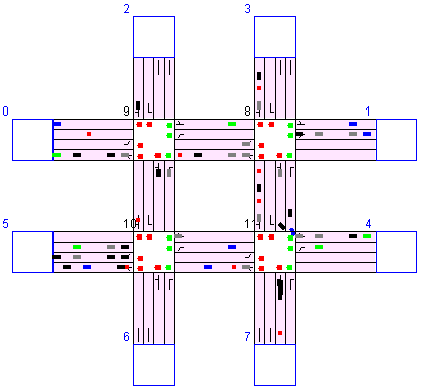
\includegraphics[width=2.3in,height=2in]{fig/2x2grid.png}
}
\\		
\subfigure[AVG-SPSA]{
\label{fig:avg}
\hspace{-2em} 
\tabl{c}{\scalebox{0.75}{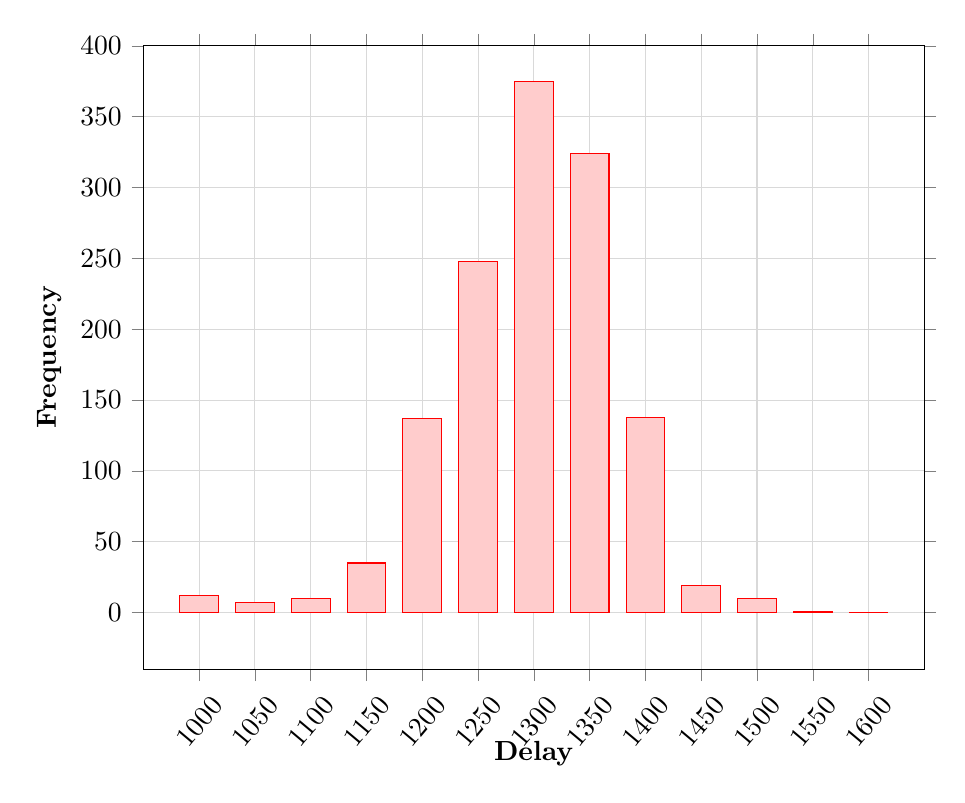
\begin{tikzpicture}
\begin{axis}[
ybar={2pt},
ymax=400,
%  legend style={at={(0.5,-0.2)},anchor=north,legend columns=-1},
legend pos=outer north east,
legend image code/.code={\path[fill=white,white] (-2mm,-2mm) rectangle
(-3mm,2mm); \path[fill=white,white] (-2mm,-2mm) rectangle (2mm,-3mm); \draw
(-2mm,-2mm) rectangle (2mm,2mm);},
ylabel={\bf Frequency},
xlabel={\textbf{Delay}},
x label style={at={(axis description cs:0.5,-0.1)},anchor=north},
symbolic x coords={0, 1000, 1050, 1100,1150,1200,1250,1300,1350,1400,1450, 1500, 1550, 1600, 14},
xmin={0},
xmax={14},
xtick=data,
ytick align=outside,
xticklabel style={rotate=50, align=center},
bar width=14pt,
% nodes near coords,
grid,
grid style={gray!30},
width=11.5cm,
height=9.5cm,
]
\addplot[red, fill=red!20]   coordinates { (1000,12) (1050,7) (1100,10)   (1150,35) (1200,137) (1250,248) (1300,375) (1350,324) (1400,138) (1450,19) (1500,10) (1550,1) (1600,0) }; 
% \addplot[red, fill=red!20]   coordinates { (1100,3) (1150,15) (1200,36) (1250,100) (1300,145) (1350,47) (1400,5) (1450,0) }; 
\end{axis}
\end{tikzpicture}}\\[0.5ex]}
}
\\
%%%%%%%%%%%%%%%%%%%%%%%%%
\subfigure[CPT-SPSA]{
\label{fig:cpt}
\hspace{-2em} 
\tabl{c}{\scalebox{0.75}{\begin{tikzpicture}
\begin{axis}[
ybar={2pt},
%  legend style={at={(0.5,-0.2)},anchor=north,legend columns=-1},
ymax=400,
legend pos=outer north east,
legend image code/.code={\path[fill=white,white] (-2mm,-2mm) rectangle
(-3mm,2mm); \path[fill=white,white] (-2mm,-2mm) rectangle (2mm,-3mm); \draw
(-2mm,-2mm) rectangle (2mm,2mm);},
ylabel={\bf Frequency},
xlabel={\textbf{Delay}},
x label style={at={(axis description cs:0.5,-0.1)},anchor=north},
symbolic x coords={0, 1000, 1050, 1100,1150,1200,1250,1300,1350,1400,1450,1500, 12},
xmin={0},
xmax={12},
xtick=data,
ytick align=outside,
xticklabel style={rotate=50, align=center},
bar width=14pt,
% nodes near coords,
grid,
grid style={gray!30},
width=11.5cm,
height=9.5cm,
]
% \addplot[darkgreen, fill=darkgreen!20]   coordinates {  (1100,16) (1150,38) (1200,69) (1250,44) (1300,51) (1350,16) (1400,22) (1450,17) (1500,24) }; 
\addplot[darkgreen, fill=darkgreen!20]   coordinates {  (1000,5) (1050,10) (1100,4) (1150,19) (1200,105) (1250,232) (1300,326) (1350,363) (1400,180) (1450,19) (1500,0) }; 
 

\end{axis}
\end{tikzpicture}}\\[0.5ex]}
}
\end{tabular}
\caption{Histogram of the delays for two SPSA-based algorithms: AVG-SPSA uses plain sample means (no utility/weights) and CPT-SPSA uses both utilites and weights. }
\label{fig:histogram-perf}
\end{figure}

We consider two different notions of return as follows:
%
\textbf{CPT:} Let $\mu^i$ be the proportion of road users along path $i$, for $i=1,\ldots,\M$. Any road user along path $i$ will evaluate the delay he experiences in a manner that is captured well by CPT. Let $X_i$ be the delay r.v. for path $i$ and let the corresponding CPT-value be $\C(X_i)$. With the objective of maximizing the experience of road users across paths, the overall return to be optimized is given by
\begin{align}
\text{CPT}(X_1,\ldots,X_{\M}) = \sum_{i=1}^{\M} \mu^i \C(X_i).\label{eq:cpt-traffic}
\end{align}
% \textbf{EUT:} Here we only use the utility functions $u^+$ and $u^-$ to handle gains and losses, but do not distort probabilities. 
% Thus, the EUT objective is defined as
% \begin{align*}
% \text{EUT}(X_1,\ldots,X_{\M}) = \sum_{i=1}^{\M} \mu^i \left(\E(u^+(X_i) - \E(u^-(X_i)\right),
% \end{align*}
% where $\E(u^+(X_i)) = \intinfinity \Prob{u^+(X_i)>z} dz$ and $\E(u^-(X_i)) - \intinfinity \Prob{u^-(X_i)>z} dz$, for $i=1,\ldots,\M$.
\textbf{AVG:} This is the usual expected value with no distinction between gains and losses via utility functions and no distortion of probabilities, i.e., 
\begin{align}
\text{AVG}(X_1,\ldots,X_{\M}) = \sum_{i=1}^{\M} \mu^i \E(X_i). 
\end{align}
%Thus, the AVG objective is defined as
%\begin{align}
%\text{AVG}(X_1,\ldots,X_{\M}) = \sum_{i=1}^{\M} \mu^i \E(X_i).
%\end{align}   
%where $\E(X_i) = \intinfinity P(u^+(X_i)>z) dz - \intinfinity P(u^-(X_i)>z) dz$.
An important component of CPT is to employ a reference point to calculate gains and losses. 
%Choosing a suitable reference point is challenging, but \cite{tversky1992advances} advocate using status-quo as the reference point. 
In our setting, we use path-wise delays obtained from a pre-timed TLC (cf. the Fixed TLCs in \cite{prashanth2011reinforcement}) as the reference point. If the delay of any TLC algorithm is less than that of pre-timed TLC, then the (positive) difference in delays is perceived as a gain and in the complementary case, the delay difference is perceived as a loss. Thus, the CPT-value $\C(X_i)$ for any path $i$ in \eqref{eq:cpt-traffic} is to be understood as a \textit{differential delay}.  

%, as the road network considered is high-dimensional (state space cardinality $> 10^{60}$). 

Using a Boltzmann policy that has the form
$$
\pi_{\theta}(s,a) = \frac{e^{\theta^{\top} \phi_{s,a}}}{\sum_{a' \in {\A(s)}} e^{\theta^{\top} \phi_{s,a'}}},
\hspace{6pt} \forall s \in \S,\;\forall a \in \A(s),
$$
with features $\phi_{s,a}$ as described in Section V-B of \cite{prashanth2012threshold},
we implement the following TLC algorithms:

{\bf\em CPT-SPSA}: This is the first-order algorithm with SPSA-based gradient estimates, as described in Algorithm \ref{alg:1spsa}. In particular, the estimation scheme in Algorithm \ref{alg:holder-est} is invoked to estimate $\C(X_i)$ for each path $i=1,\ldots,\M$, with $d_n^{i,j}, j=1,\ldots,n_i$ as the samples.

% {\bf\em EUT-SPSA}: This is similar to CPT-SPSA, except that weight functions $w^+(p)=w^-(p)=p,$ for $p\in [0,1]$. 

{\bf\em AVG-SPSA}: Here we employ SPSA to update the policy parameter in the descent direction, with sample averages of the delays as input. 

For CPT-SPSA, we set the utility functions (see \eqref{eq:cpt-general}) as follows:
$$u^+(x) =  |x|^{\sigma}, \text{ and  }u^-(x) = \lambda |x|^{\sigma},$$ 
where $\lambda = 2.25$ and $\sigma = 0.88$.
The weight functions $w^+,w^-$ have the formas set as follows:
\begin{align*}
w^+(p) &= \frac{p^{\eta_1}}{{(p^{\eta_1}+ (1-p)^{\eta_1})}^{\frac{1}{\eta_1}}}, w^-(p) = \frac{p^{\eta_2}}{{(p^{\eta_2}+ (1-p)^{\eta_2})}^{\frac{1}{\eta_2}}},
\end{align*} 
where $\eta_1 = 0.61$ and $\eta_2 = 0.69$. The choices for $\lambda$, $\sigma$, $\eta_1$ and $\eta_2$ are based on median estimates given by \cite{tversky1992advances} and have been used earlier in a traffic application (see \cite{gao2010adaptive}).
For all the algorithms,
 motivated by standard guidelines (see \cite{spall2005introduction}),
 we set $\delta_n = 1.9/n^{0.101}$ and $a_n = 1/(n+50)$. The initial point $\theta_0$ is the $d$-dimensional vector of ones and $\forall i$, the operator $\Gamma_i$ keeps the iterate $\theta_i$ bounded within $[0.1, 1.0]$.

\begin{table}
 \centering
 \begin{tabular}{c|c|c}
  \toprule 
   & \textbf{Expected value}& \textbf{CPT-value }\\\midrule
   AVG-SPSA & $1596.55$ & $624.68$ \\\midrule
   CPT-SPSA & $1744.94$ & $659.61$\\
   \bottomrule
  \end{tabular}
  \caption{AVG and CPT-value estimates for AVG-SPSA and CPT-SPSA algorithms. Note: CPT-value is of differential delays w.r.t. pre-timed TLC, while expected value uses plain delays.}
  \label{tab:cpt-results}
\end{table}

 
The experiments involve two phases:
first, a training phase where we run each algorithm for $500$ iterations, with each iteration involving two perturbed simulations. Each simulation involves running the traffic simulator with a fixed policy parameter for $2000$ steps and this corresponds to approximately $2000$ delay samples. The training phase is followed by a test phase where we fix the policy obtained at the end of training (i.e., after $500$ steps of SPSA) and then run the traffic simulator with the aforementioned parameter for $30000$ steps. 

% \subsection{Results} 

Figures \ref{fig:avg}--\ref{fig:cpt} present the histogram of the delays obtained from the test phase for AVG-SPSA and CPT-SPSA, respectively.  
% A similar exercise for pre-timed TLC resulted in a CPT-value of $-46.14$. 
It is evident that each algorithm converges to a different policy and the difference, in $\ell_1$ norm, between policy parameters obtained at the end of training phase for AVG-SPSA and CPT-SPSA was $4.93$. 
As shown in Table \ref{tab:cpt-results},  AVG-SPSA results in a TLC policy with lower expected delay, while CPT-SPSA's policy has higher CPT-value. This is expected because AVG-SPSA uses neither utilities nor probability distortions and minimizes overall delay, while CPT-SPSA uses a pre-timed TLC baseline and treats delay gains and losses differently. 
Interestingly, CPT-SPSA results in a policy that has a distribution which is more spread out, i.e., with heavier tail, as compared to AVG-SPSA and this is apparent from Figures \ref{fig:avg}--\ref{fig:cpt}. 

The results in this as well as previous section argue for specialized algorithms that incorporate CPT-based criteria, esp. in the light of previous findings which show CPT matches human evaluation well and there is a need for algorithms that serve human needs well.
%\todoc{It would be nice to point out how the CPT policy is different than the others.}



%%%%%%%%%%%%%%%%%%%%%%%%%%%%%%%%%%%%%%%%%%%%%%%%%%%%%%%%%%%%%%
%%%%%%%%%%%%%%%%%%%%%%%%%%%%%%%%%%%%%%%%%%%%%%%%%%%%%%%%%%%%%%
%%%%%%%%%%%%%%%%%%%%%%%%%%%%%%%%%%%%%%%%%%%%%%%%%%%%%%%%%%%%%%
%%%%%%%%%%%%%%%%%%%%%%%%%%%%%%%%%%%%%%%%%%%%%%%%%%%%%%%%%%%%%%


\section{Conclusions}
\label{sec:conclusions}
CPT has been a very popular paradigm for modeling human decisions among psychologists/economists, but has escaped the radar of the reinforcement learning community. This work is the first step in incorporating CPT-based criteria into an RL framework. However, both prediction and control of CPT-based value is challenging. 
%Using temporal-difference learning type algorithms for estimation was ruled out for CPT-value since the underlying probabilities get (non-linearly) distorted by a weight function. 
For prediction, we proposed a quantile-based estimation scheme. Next, for the problem of control, since CPT-value does not conform to any Bellman equation, we employed SPSA - a popular simulation optimization scheme and designed a first-order algorithm for optimizing the CPT-value. 
We provided theoretical convergence guarantees for all the proposed algorithms and illustrated the usefulness of our algorithms for optimizing CPT-based criteria in a traffic signal control application.

%%%%%%%%%%%%%%%%%%%%%%%%%%%%%%%%%%%%%%%%%%%%%%%%%%%%%%%%%%%%


%\subsubsection*{Acknowledgments}
%This work was supported by the Alberta Innovates Technology Futures through the Alberta Ingenuity Centre for Machine Learning, NSERC, the National Science Foundation (NSF) under Grants CMMI-1434419, CNS-1446665, and CMMI-1362303, and by the Air Force Office of Scientific Research (AFOSR) under Grant FA9550-15-10050.
%
%\clearpage
%\newpage

%%%%%%%%%%%%%%%%%%%%%%%%%%%%%%%%%%%%%%%%%%%%%%%%%%%%%%%%%%%%%%%%%%%%%%%%%%%%%%%%%%%%%%%%%%%%%%%%%%%%%%%%%%%%%%%%%%%%%%%%%%%%%%%%%%%%%%
\bibliographystyle{IEEEtran}
\bibliography{cpt-refs}

 %\section*{Appendix}

%%!TEX root =  cpt-rl-icml.tex


\appendix

%%%%%%%%%%%%%%%%%%%%%%%%%%%%%%%%%%%%%%%%%%%%%%%%%%%%%%%%%%%%%%

%%%%%%%%%%%%%%%%%%%%%%%%%%%%%%%%%%%%%%%%%%%%%%%%%%%%%%%%
\section{Background on CPT}
\label{sec:appendix-cpt-intro}
\todoc[inline]{Is this section referred to from the main text?}
The purpose of this appendix is to explain the ideas underlying CPT. 
To avoid technicalities we will do this in the context of discrete random variables.
Let $X$ be a discrete valued random variables, taking values in $\{x_1,\dots,x_K\}$ (the set of possible ``prospects'') 
and let $p_i = \Prob{X=x_i}$.
We shall think of $X$ as a random loss or gain incurred by a human decision maker.
%For a random variable $X$ taking values in $\{x_1,\dots,x_K\}$, let $p_i, i=1,\ldots,K$ denote the probability of incurring a gain/loss $x_i, i=1,\ldots,K$. %Assume $x_1 \le \ldots \le x_K$. 
Given a utility function $u:\R\rightarrow \R_+:[0,1] \rightarrow [0,1]$ and weighting function $w$, \todoc{What is the domain and range of these functions?}
the \textit{\textbf{prospect theory}} (PT) value of $X$ is defined as 
\begin{align}
\C(X) = \sum_{i=1}^K u(x_i) w(p_i).
\label{eq:ptval}
\end{align} 
The idea is to take an utility function that is $S$-shaped, so that it satisfies the \textit{diminishing sensitivity}  property. 
If we take the weighting function $w$ to be the identity, then one recovers the classic expected utility. A general weight function inflates low probabilities and deflates high probabilities and this has been shown to be close to the way humans make decisions. 
In \cite{kahneman1979prospect} and \cite{fennema1997original}, the authors present justification of PT in the form of experimental results  using human subjects.
%However, distorting the probabilities via a weighting function (that is not identity) is a useful generalization since it  overcomes some of the ill-effects of expected utility and is closer to human decision making - see \cite{kahneman1979prospect}. 

However, the weight function in PT  lacking in some theoretical aspects as it violates first-order \textit{stochastic dominance}. We illustrate this via the following example: Consider a prospect, say P1, where outcomes $10$ and $0$ occur with probabilities $0.1,  0.9$, respectively. Let P2 be another prospect  where the outcomes are $10, 10+\epsilon$ and $0$, with respective probabilities $0.05$, $0.05$ and $0.9$.

The weight function $w$ is non-additive as it is non-linear and since $0.05$ and $0.1$ are in the low-probability regime, we can assume that $w(0.1) > 2 w(0.05)$. Suppose $\epsilon>0$ be small enough such that $w(0.1) > (2+\epsilon) w(0.05)$. Then, the PT-value, as defined in \eqref{eq:ptval}, of P1 is higher than that of P2 and hence, P1 is preferred.

On the other hand, P2 stochastically dominates P1, where stochastic dominance is defined as follows:
A prospect ${\cal B}$ stochastically dominates prospect ${\cal A}$ if the probability of receiving a value $x$ or greater is at least as high under prospect ${\cal B}$ as it is under prospect ${\cal A}$  for all values of $x$, and is strictly greater for some value of $x$.
  
\todoc{What does ``it'' refer to here? Consider rephrasing this}  \todoc{Why is this true??}
\todoc{What does ``this'' refer to here?}
%Thus, 
%violates stochastic dominance, since a shift in the probability mass from bad outcomes does not result in a better prospect.  
\todoc{This is hard to understand; consider rephrasing it more clearly.}

\textbf{Cumulative prospect theory} (CPT) \cite{tversky1992advances} uses a similar measure as PT, except that the weights are a function of cumulative probabilities. First, separate the gains and losses as 
$x_1\le \ldots \le x_l \le 0 \le x_{l+1} \le \ldots \le x_K$,
where zero is used as an arbitrary reference point.
Then, the CPT-value of $X$ is defined as 
\begin{align*}
\C(X) &= u^-(x_1)\cdot w^-(p_1) + u^+(x_K)\cdot w^+(p_K)\\
&\quad+\sum\limits_{i=2}^l u^-(x_i) \Big(w^-(\textstyle\sum\limits_{j=1}^i p_j) - w^-(\textstyle\sum\limits_{j=1}^{i-1} p_j)\Big)  \\
&\quad 
 + \sum\limits_{i=l+1}^{K-1} u^+(x_i) \Big(w^+(\textstyle\sum\limits_{j=i}^K p_j) - w^+(\textstyle\sum\limits_{j=i+1}^K p_j) \Big), 
\end{align*} 
where $u^+, u^-$ are utility functions and $w^+, w^-$ are weight functions to distort gains and losses, respectively. The utility functions $u^+$ and $u^-$ are non-decreasing, while the weight functions are continuous, non-decreasing and have the range $[0,1]$ with $w^+(0)=w^-(0)=0$ and $w^+(1)=w^-(1)=1$ . 
Unlike PT, the CPT-value does not violate first-order stochastic dominance, as the weight functions act on cumulative probabilities. 
%In the aforementioned example, increasing $w^-(0.05)$ and $w^+(0.05)$ \todoc{Or the probabilities of the corresponding outcomes!?}
%does not impact outcomes other than those on the extreme, i.e., $-10$ and $180$, respectively. For instance, the weight for outcome $100$ would be $w^+(0.45) - w^+(0.40)$. \todoc{When?}
%Thus, \todoc{Why is this a corollary of the previous paragraph?}
%CPT formalizes the intuitive notion that humans are sensitive to extreme outcomes and relatively insensitive to intermediate ones.

\subsection*{Allais paradox}
Allais paradox is not as much as a paradox, but an argument that shows that 
expected utility theory is inconsistent with human preferences.
Suppose we have the following two traffic light switching policies:

\textbf{\textit{[Policy 1]}} A throughput (number of vehicles that reach destination per unit time) of $1000$  w.p. $1$. Let this be denoted by $(1000,1)$.

\textbf{\textit{[Policy 2]}}  $(10000, 0.1; 1000,0.89; 100, 0.01)$ i.e., throughputs $10000$, $1000$ and $100$ with respective probabilities $0.1$, $0.89$ and $0.01$.

Humans usually choose Policy $1$ over Policy $2$. On the other hand, consider the following two policies:

\textbf{\textit{[Policy 3]}} (100, 0.89; 1000, 0.11)

\textbf{\textit{[Policy 4]}} (100, 0.9; 10000, 0.1)

Humans usually choose Policy $4$ over Policy $3$. 

We can now argue against using expected utility (EU) as an objective as follows
accepting the above preferences: Let $u$ be the utility function in EU.
Since Policy 1 is preferred over Policy 2,
$u(1000) > 0.1 u(10000) + 0.89 u(1000) + 0.01 u(100)$, which is equivalent to
\begin{align}
0.11 u(1000) > 0.1 u(10000) + 0.01 u(100)\,.
 \label{eq:12}
\end{align}
On the other hand, since Policy 4 is preferred over Policy 3, 
$0.89 u(100) + 0.11 u(1000) < 0.9 u(100) + 0.1 u(10000)$, which is equivalent to
\begin{align}
 0.11 u(1000) < 0.1 u(10000) + 0.01 u(100) \,.\label{eq:23}
\end{align}
Now note that  \eqref{eq:12} contradicts \eqref{eq:23}. Hence, no utility function exist that is consistent with human preferences.

%\newpage
%%%%%%%%%%%%%%%%%%%%%%%%%%%%%%%%%%%%%%%%%%%%%%%%%%%%%%%%%%%%%%
%%%%%%%%%%%%%%%%%%%%%%%%%%%%%%%%%%%%%%%%%%%%%%%%%%%%%%%%%%%%%%
%%%%%%%%%%%%%%%%%%%%%%%%%%%%%%%%%%%%%%%%%%%%%%%%%%%%%%%%%%%%%%%%%%%%%%%%%%%%%%%%
%%%%%%%%%%%%%%%%%%%%%%%%%%%%%%%%%%%%%%%%%%%%%%%%%%%%%%%%%%%%%%%%%%%%%%%%%%%%%%%%
\section{CPT-value in a Stochastic Shortest Path Setting}
\label{sec:cpt-ssp}
We consider a stochastic shortest path (SSP) problem with states $\S=\{0,\ldots,\L\}$, where $0$ is a special reward-free absorbing state.  A randomized policy $\pi$ is a function that maps any state $s\in \S$ onto a probability distribution over the actions $\A(s)$ in state $s$. As is standard in policy gradient algorithms, we parameterize $\pi$ and assume it is continuously differentiable in its parameter $\theta \in \R^d$.  
An \textit{episode} is a simulated sample path using policy $\theta$ that starts in state $s^0\in \S$, visits $\{s_1,\ldots, s_{\tau-1}\}$ before ending in the absorbing state $0$, where $\tau$ is the first passage time to state $0$.
Let $D^\theta(s^0)$ be a random variable (r.v) that denote the total reward from an episode, defined by
$$ D^\theta(s^0) = \sum\limits_{m=0}^{\tau-1} r(s_m,a_m), $$
where the actions $a_m$ are chosen using policy $\theta$ and $r(s_m, a_m)$ is the single-stage reward in state $s_m\in \S$ when action $a_m \in \A(s_m)$ is chosen. 

Instead of the traditional RL objective for an SSP of maximizing the expected value $\E (D^\theta(s^0))$, 
we adopt the CPT approach and aim to solve the following problem: 
$$ \max_{\theta \in \Theta} \C(D^\theta(s^0)),$$
where $\Theta$ is the set of admissible policies that are \textit{proper}\footnote{A policy $\theta$ is proper if $0$ is recurrent and all other states are transient for the Markov chain underlying $\theta$. It is standard to assume that policies are proper in an SSP setting - cf. \cite{bertsekas1995dynamic}.} and the CPT-value function $\C(D^\theta(s^0))$ is defined as
\begin{align}
\C(D^\theta(s^0))& = \intinfinity w^+\left(\Prob{u^+(D^\theta(s^0))>z}\right) dz \nonumber
\\&- \intinfinity w^-\left(\Prob{u^-(D^\theta(s^0))>z}\right) dz. \label{eq:cpt-mdp}
\end{align}


%%%%%%%%%%%%%%%%%%%%%%%%%%%%%%%%%%%%%%%%%%%%%%%%%%%%%%%%%%%%%%%%%%%%%%%%%%%%%%%%
%\newpage


%%%%%%%%%%%%%%%%%%%%%%%%%%%%%%%%%%%%%%%%%%%%%%%%%%%%%%%%%%%%%%%%%%%%%%%%%%%%%%%%%%%%%%%%%%%%%%%%%%%%%%%%%%%%%%%%%%%%%%%%%%%%%%%
%%%%%%%%%%%%%%%%%%%%%%%%%%%%%%%%%%%%%%%%%%%%%%%%%%%%%%%%%%%%%%%%%%%%%%%%%%%%%%%%%%%%%%%%%%%%%%%%%%%%%%%%%%%%%%%%%%%%%%%%%%%%%%%

\end{document}


